\documentclass[11pt,a4paper]{article}
\usepackage[T1]{fontenc}
\usepackage[utf8]{inputenc}
\usepackage{mathptmx}
usepackage{courier}
\usepackage{amsmath}
\usepackage{graphicx}
\usepackage{booktabs}
\usepackage{array}
\usepackage{tabularx}
\usepackage{adjustbox}
\usepackage{placeins}
\usepackage{float}
\usepackage[margin=2.2cm]{geometry}
\usepackage[authoryear,round]{natbib}
\usepackage{microtype}
\usepackage[font=small,labelfont=bf]{caption}
\usepackage{xurl}
\usepackage{xcolor}
\usepackage[hidelinks]{hyperref}
\usepackage{authblk}
\urlstyle{same}
\usepackage{lineno}
\linenumbers
\renewcommand{\linenumberfont}{\normalfont\tiny\color{gray}}
\newcolumntype{L}{>{\raggedright\arraybackslash}X}
\newcolumntype{P}[1]{>{\raggedright\arraybackslash}p{#1}}
\setlength{\bibsep}{1pt plus 1pt}
\renewcommand{\bibfont}{\footnotesize}
\renewcommand{\topfraction}{0.92}\renewcommand{\bottomfraction}{0.8}\renewcommand{\textfraction}{0.06}\renewcommand{\floatpagefraction}{0.85}
\setcounter{topnumber}{3}\setcounter{totalnumber}{4}
\emergencystretch=2em

\title{The value of nuclear capacity in a zero-emission Italian power system: a capacity expansion analysis with one cost rule for every technology}
\author{Claudio Gratton}
\affil{Independent researcher, Italy}
\date{Preprint, version 8, November 2026}

\begin{document}
\maketitle

\begin{abstract}
\noindent We estimate how much nuclear capacity the least-cost Italian power system with zero direct emissions contains for a 2040 demand of 400\,TWh, with a capacity expansion model. Every technology, nuclear included, follows one cost rule (overnight cost, interest during construction, capital recovery, fixed operating cost) at today's contract or plant price without contingency, because the decision is taken now. The central nuclear cost is the Dukovany contract price plus owner's costs, 10{,}200\,EUR/kW net, the bottom of the bracket reported by the European Commission, because a plan is made to build well and the same rule applies to every technology; the rest of the bracket is read as cost cases. It is 911\,EUR/kW-yr at a 5\% real cost of capital. Trade is a balanced annual swap with no foreign capacity in the critical weeks, a planning standard: a national plan must work if every neighbour planned the same way. The critical weeks fall between November and February, when Italy's suppliers need their own firm capacity, much of it nuclear. The result is a value curve, on which any nuclear cost case is read. At 5\% the optimum is 23.2\,GW (44.5\% of demand) with technologies without commercial plants at first-plant costs and 15.7\,GW (30.5\%) with them at target costs; at 7\%, 15.6 and 11.1\,GW, the latter all small modular reactors. The optimum is flat: with first-plant costs at 5\% every capacity between 16 and 28\,GW costs within 1\% of the minimum. Counting 38\% of foreign capacity as firm in the critical weeks, with the annual balance kept, gives 17.9 and 14.1\,GW; the previous version's trade rule, a bundle of five changes that also drops the annual balance, 11.9 and 7.2\,GW. About 15\,GW is in or near the optimum in most of the cost cases from the contract cost upward, not all (16\,GW is within 1\% of the minimum in 11 of the 20 combinations of five cost cases from the contract cost upward and four curves), under three conditions: construction at the contract cost, nuclear financed at about the same real rate as the alternatives, and no foreign capacity in the critical weeks.
\end{abstract}

\noindent\textbf{Keywords:} nuclear power; capacity expansion; Italy; system cost; value curve; cost of capital; import dependence

\medskip
\noindent\textbf{Highlights}
\begin{itemize}\setlength\itemsep{0pt}
\item One cost rule for every technology, nuclear included, at today's contract or plant price without contingency, because the decision is taken now; auction prices are not costs.
\item The result is a value curve of nuclear capacity, from which any nuclear cost case is read.
\item Optimum at 5\%: 23.2\,GW with technologies without commercial plants at first-plant costs, 15.7\,GW with them at target costs.
\item The optimum is flat: 16 to 28\,GW cost within 1\% of the minimum with first-plant costs at 5\%.
\item Counting 38\% of foreign capacity as firm in the critical weeks, with the annual balance kept, gives 17.9 and 14.1\,GW; the previous version's trade rule, a bundle of five changes that also drops the annual balance, gives 11.9 and 7.2\,GW.
\item About 15\,GW needs construction at the contract cost, nuclear financed at about the same real rate as the alternatives, and no foreign capacity in the critical weeks.
\end{itemize}

\section{Introduction}\label{sec:intro}

In 2026 the Italian Parliament gave final approval to a law that delegates to the government the reintroduction of nuclear power \citep{Delega2026}. The law authorises no plant and selects no site. How much nuclear capacity a zero-emission Italian power system should contain, and under which conditions, is therefore a practical question.

The public debate relies mostly on the levelised cost of electricity (LCOE), by which utility-scale solar photovoltaics (PV) is much cheaper than new nuclear \citep{IEA2024WEO,FraunhoferEN2024}. The LCOE divides the cost of a plant by the energy it produces, regardless of when it produces it, so it does not measure the cost of meeting demand in every hour. System studies do: \citet{Sepulveda2018} find that firm low-carbon resources lower the cost of fully decarbonised power systems by 10--62\%. For Italy, \citet{Lombardi2020} describe near-optimal systems based on solar, wind and synthetic fuels, without nuclear; \citet{Mastrantuono2026} find that new nuclear lowers total system cost, in a model where nuclear capacity has an exogenous cap, so the optimal amount is not identified.

A second problem is the stability of the answer. Earlier versions of the present study gave a nuclear share between 74\% and 29\% of demand as inputs and rules were corrected (Section~\ref{sec:trajectory}), so the result must be stated in a form that shows why it moves.

This paper makes four contributions.
\begin{enumerate}\setlength\itemsep{1pt}
\item \emph{One cost rule for every technology, nuclear included.} The annual cost of each technology is its overnight cost times interest during construction and the capital recovery factor over its technical life, plus fixed operating cost. Costs are those of plants, most of them contracted or built in 2024--2026, from official or regulatory sources where they exist and otherwise from university, industry or press sources, each named with its input. Auction prices are not used as costs, because they can be combined with grants or rely on revenues outside the contract.
\item \emph{The result as a value curve of nuclear capacity.} Runs with nuclear capacity fixed at $N$ give the system cost $C(N)$ and, from it, the annual fixed cost at which each further block of capacity is worth building. The curve does not depend on the cost assumed for nuclear, so any cost case is read on it, and it shows how flat the optimum is.
\item \emph{Trade as a balanced swap.} In the central rule Italy imports as much as it exports in every year and gets no energy and no capacity credit from abroad in the critical weeks. The critical weeks all fall in winter, when the countries that supply 85\% of Italy's imports need their own firm capacity, much of it nuclear; a system without Italian nuclear that relies on them is not a system without nuclear. We also report the result and the system cost under a rule close to today's import dependence.
\item \emph{Open code, data and a full error register.} The repository holds the model, every input with its source, one result line per run and the register of the 98 errors found in the project so far (Appendix~\ref{app:audit}).
\end{enumerate}

The model describes a steady-state system, with 2040 demand and all fleets already built; it is not a transition path. It has one node. Section~\ref{sec:methods} describes the model, the cost rule and the value-curve method, Section~\ref{sec:results} the results, Section~\ref{sec:discussion} discusses them and lists the limitations with the direction of their bias, and Section~\ref{sec:conclusions} concludes.

\section{Methods and data}\label{sec:methods}

\subsection{Capacity expansion model}\label{sec:model}
The model is a linear programme that chooses the capacities and the dispatch of all technologies so as to meet demand in every time step at least cost, with zero direct emissions. It has one node. One fleet must serve the four weather years 2016--2019, which are optimised together, with a three-hour step: 11{,}680 steps, 315{,}000 to 390{,}000 variables and 365{,}000 to 475{,}000 constraints (about twice with eight weather years) per run. It is solved with HiGHS \citep{HiGHS}; all runs reported here ended with status optimal. The decision variables are the capacities of solar photovoltaics (PV: ground-mounted, agrivoltaic, industrial and other roofs, by zone, with finite land), onshore and offshore wind (finite blocks), large nuclear reactors, small modular reactors (SMRs), batteries, hydrogen (electrolyser, underground storage, turbine), compressed air, 100-hour storage, new pumped hydro, new hydropower, geothermal, bioenergy, concentrated solar power with storage (CSP), interruptible load, smart charging and new interconnection. Existing hydropower (15\,GW, 43.4\,TWh a year) and pumped hydro are given.

With $K_i$ the capacity of technology $i$, $c_i$ its annual fixed cost (Section~\ref{sec:rule}), $g_{i,t}$ its output in step $t$ with variable cost $v_i$, $m_t$ imports and $x_t$ exports, the objective over $Y=4$ years is
\begin{equation}
\min\; Y\sum_i c_i K_i+\sum_t\Big(\sum_i v_i\,g_{i,t}+p_m\,m_t-p_x\,x_t\Big),
\end{equation}
with import price $p_m=115.94$\,EUR/MWh, the 2025 average Italian price, and export revenue $p_x=61.07$\,EUR/MWh, the 2025 average French price \citep{GME2025}. The energy balance in each step of length $\Delta$ is
\begin{equation}
\sum_i g_{i,t}+\sum_s\big(d_{s,t}-q_{s,t}\big)+m_t-x_t+u_t=L_t ,\label{eq:balance}
\end{equation}
where $d_{s,t}$ and $q_{s,t}$ are discharge and charge of storage $s$, $u_t$ is the net effect of demand shifting and $L_t$ is demand. Solar and wind output is bounded by the profile, $g_{b,t}\le K_b\,\rho_b\,s_t$ for block $b$ with scale $\rho_b$, so curtailment is free. Nuclear output moves between a minimum and a maximum share of the available capacity,
\begin{equation}
\mu\,a_t\,N\Delta\le n_t\le a_t\,N\Delta ,
\end{equation}
with minimum load $\mu=0.5$ and a monthly availability $a_t$ whose shape is an assumption: 95\% in the winter and summer months, less in spring and autumn, with a mean of 90\%, the load factor in the Commission decision on Dukovany (15.4\,TWh a year on 1{,}952\,MW; \citealp{ECDukovany2026}). Each storage follows
\begin{equation}
e_{t+1}=e_t+\eta\,q_t-d_t,\qquad 0\le e_t\le E,\qquad q_t,\,d_t\le E\Delta/\tau ,
\end{equation}
with efficiency $\eta$, duration $\tau$ and cyclic levels; hydrogen has separate capacities for electrolyser, store and turbine. Hydropower must produce a given energy $H_m$ in each month $m$, with a minimum flow equal to 37\% of the monthly mean and a maximum power of 15\,GW; the monthly budgets are the same in every weather year. There are no ramp constraints.

\paragraph{Adequacy.} Firm capacity must be at least 1.1 times the peak load:
\begin{equation}
\sum_i \kappa_i K_i\ge 1.1\,\hat L ,\qquad \hat L=76.9\ \mathrm{GW},
\end{equation}
where $\hat L$ is the peak of the three-hour data and is used at every time step, so the requirement (84.6\,GW, our calculation) does not change when the model is run at a coarser step. The credits $\kappa_i$ are assumptions: nuclear, geothermal and new hydropower at their availability; existing hydro (15\,GW), existing and new pumped hydro, compressed air and 100-hour storage at full power; batteries at their power times 4/6.6; hydrogen turbines and bioenergy at 0.95; interruptible load at 1.0; CSP from its profile in the highest load steps; solar PV, wind and imports at zero.

\paragraph{Trade.} Imports use the interconnection capacity $I$, which is 11{,}535\,MW today \citep{ARERA366} and can be expanded with up to 7.33\,GW of new lines at their cost. Exports have their own variable in the balance~\eqref{eq:balance} and are limited to a fraction of the import capacity, the ratio of the export and import limits of Terna, the grid operator \citep{TernaCapObj2025}:
\begin{equation}
x_t\le \frac{6{,}095}{11{,}535}\,I\,\Delta .
\end{equation}
Annual trade is balanced in each weather year $y$ with demand $D_y$:
\begin{equation}
-X_{\mathrm{exp}}\,D_y\;\le\;\sum_{t\in y}\big(m_t-x_t\big)\;\le\;X\,D_y ,\qquad X=X_{\mathrm{exp}}=0 ,\label{eq:swap}
\end{equation}
so in the central rule Italy is neither a net importer nor a net exporter: it swaps energy with its neighbours, paying 115.94 and earning 61.07\,EUR/MWh. In the critical weeks imports are not available ($m_t=0$) and interconnection has no capacity credit. The critical weeks are the three weeks of each year with the highest mean residual load, defined as load minus the output of a reference mix of 100\,GW of PV and 40\,GW of onshore wind. The reason for the rule is that the plan must work if every neighbour planned the same way. Today Italy depends on imports (55.2\,TWh imported and 7.4 exported in 2025; \citealp{GME2025}), and Section~\ref{sec:dependence} explains why the rule is needed to compare systems with and without nuclear (in the critical weeks the foreign firm capacity is largely nuclear) and gives the cost of ending the dependence. The neighbouring systems are not simulated.

\paragraph{Grid.} Every new solar and onshore wind kilowatt pays a transmission charge of 13\,EUR/MWh at 1{,}066 hours (PV) or 8\,EUR/MWh at 1{,}709 hours (wind), about 240\,EUR/kW over 40 years; nuclear pays 2\,EUR/MWh and offshore wind no per-MWh charge. New capacity above a total wind and PV stock of 137\,GW, offshore wind included, pays a second charge of 13.77\,EUR/kW-yr, about 236\,EUR/kW. The model keeps 37.8\,GW of existing plants (24.2\,GW of PV and 13.6\,GW of onshore wind), so the second charge starts at 99.2\,GW of new plants. The charges and the threshold are assumptions of the authors, not figures of the grid operator. In the PI system without nuclear 118\,GW pay the second charge (4.57\,EUR/MWh), and the average over all new PV and wind is about 363\,EUR/kW. Terna's 2025 development plan, over EUR\,23 billion for 65\,GW more renewables by 2030 on the 43\,GW installed in 2023 \citep{TernaPdS2025}, implies about 350\,EUR/kW on average for those 65\,GW; the plan also serves security and demand, but it does not cover the new PV and wind of the 2040 systems, up to about 217\,GW in the PI system without nuclear, whose integration cost is not known. Whether our charge is higher or lower than the real one is not established; a check with about 340\,EUR/kW on every new kilowatt and the second charge above 108\,GW gives 26.7\,GW in PI and 19.1\,GW in OB (three-hour runs). The charge follows the discount rate like every other capital cost. Distribution grids are not costed.

\paragraph{Demand and profiles.} Demand is 400\,TWh: a base of 338\,TWh, 15\,TWh of heat pumps and 47\,TWh of electric vehicles, just below the 404--439\,TWh of the Terna and Snam scenario report \citep{DDS2024}. The base follows the Terna load of 2016--2019, paired with the same weather year; solar and wind capacity factors are those of the Pan-European Climatic Database \citep{PECD2021}. New ground-mounted and agrivoltaic plants have trackers, with a yield 1.12 times the fixed-tilt profile, and degradation of 0.5\% a year lowers the mean output over the life to 0.94 of the first year. Existing PV and onshore wind plants pay operating cost only; the PV yield is scaled to the 1{,}117 hours of the national fleet in 2025 \citep{GSEPV2025} and existing wind runs 1{,}600 hours. System costs are divided by the 356.6\,TWh of demand not met by existing hydropower. The nuclear share is nuclear output over total demand, so it includes the nuclear energy exported in the swap.

\subsection{One cost rule for every technology}\label{sec:rule}
The annual fixed cost per unit of capacity is
\begin{equation}
c_i=K^{\mathrm{on}}_i\;\phi(r,T_i)\;\mathrm{CRF}(r,L_i)+F_i ,\qquad
\phi(r,T)=\frac1T\sum_{k=0}^{T-1}(1+r)^{T-k-1/2},\qquad
\mathrm{CRF}(r,n)=\frac{r(1+r)^n}{(1+r)^n-1},\label{eq:rule}
\end{equation}
where $K^{\mathrm{on}}_i$ is the overnight cost, with development and grid connection included and contingency, subsidies and grants excluded, $\phi$ is interest during construction with uniform spending over the build time $T_i$, CRF the capital recovery factor over the technical life $L_i$, $F_i$ the fixed operation and maintenance (O\&M) cost and $r$ the real cost of capital, 5\% in the central case and 7\% as the alternative, the same for every technology. Costs are in real 2025 euros, per unit of net capacity and with realistic output. There is no cost decline to 2040, except in the target case defined below. The decision is taken now: nuclear must be contracted now, at today's prices, because it takes about ten years from decision to operation. The alternatives are compared in the same way: PV and batteries are built in one or two years, and the hydrogen that would replace nuclear in the winter weeks is the last part of the system, built just before fossil plants close. Future costs for the alternatives only would compare a contract with a forecast; future costs for all, nuclear series included, would compare two forecasts. Three inputs are annual prices and do not go through Eq.~\eqref{eq:rule}: hydrogen storage, 100-hour storage and interruptible load.

The sources differ in kind (Table~\ref{tab:inputs} and Appendix~\ref{app:inputs}). Official or regulatory documents give the nuclear contract price, build time and operating cost (the Commission decision), the cost of batteries and of interruptible load (the regulator ARERA), the cost of roof PV and of wind and the O\&M of PV (a study of the state agency GSE for ARERA) and the cost of electrolysers (the International Energy Agency, IEA). A university report (Politecnico di Milano) and an industry association (Italia Solare) give the cost of ground-mounted and agrivoltaic PV and of wind. Press sources give the owner's costs of Dukovany and the cost of SMRs. Studies, single projects or makers' targets give hydrogen storage, compressed air and 100-hour storage. Most costs are of plants contracted or built in 2024--2026; the first-plant cost of CSP (Andasol, 2008) and the Barakah cost case (a 2009 contract) are older and revalued.

Auction prices are not used as costs. The price of the first auction of FER-X, the Italian scheme of two-way contracts for renewables, was 56.82\,EUR/MWh for solar \citep{FERXmain2025}; it can be combined with capital grants of up to 40\%, in which case the tariff is cut by up to 35\%, and with tax credits \citep{AndersenFERX}. The price of the first auction of MACSE, the Italian mechanism that procures storage capacity, was 12{,}959\,EUR/MWh-yr, and according to analysts it relied on revenues after the contract and on low returns \citep{ModoMACSE}.

\begin{table}[!tb]
\centering\footnotesize
\caption{Main cost inputs under the common rule; annual cost at 5\% from Eq.~\eqref{eq:rule}; life and build time in years. Nuclear operating expenditure (OPEX) of 40\,EUR/MWh is 27.75 fixed (at a 90\% load factor) and 12.25 variable. Sources: EC+TV, contract price in \citet{ECDukovany2026} plus owner's costs from \citet{CT24Dukovany}; PM, \citet{PoliMiRER2025}; IS, \citet{ItaliaSolare2025}; GSE, \citet{GSELCOE2025}; PVPS, \citet{IEAPVPS2024}; AR, \citet{ARERA332}; IEA, \citet{IEAGHR2025}; HY, \citet{HystoriesD86}; DA, Darlington BWRX-300 \citep{POWERDarlington2025}. Roof PV: mean of GSE (850) and PM (1{,}000--1{,}100) for industrial roofs, of GSE (1{,}100) and PVPS (1{,}400) for other roofs. Batteries: 150.5\,EUR/kWh times 1.12 for oversizing, 85\% round-trip efficiency. No floating offshore plant has been built in Italy. The other inputs are in Appendix~\ref{app:inputs}.}\label{tab:inputs}
\begin{tabularx}{\linewidth}{@{}P{3.15cm}P{2.95cm}P{2.55cm}P{0.8cm}P{3.0cm}L@{}}
\toprule
Technology & Overnight cost & Fixed O\&M & Life, build & Annual cost at 5\% & Source\\
\midrule
Large nuclear (central) & 10{,}200\,EUR/kW net & OPEX 40\,EUR/MWh & 60, 9 & 911\,EUR/kW-yr (1{,}239 at 7\%) & EC+TV\\
SMR, first plant (PI) & 17{,}200\,EUR/kW & as nuclear (proxy) & 60, 5 & 1{,}264\,EUR/kW-yr & DA, unit 1\\
SMR, target (OB) & 11{,}700\,EUR/kW & as nuclear (proxy) & 60, 5 & 934\,EUR/kW-yr (1{,}231 at 7\%) & DA, four units\\
PV ground, tracker & 950\,EUR/kWp & 20\,EUR/kWp-yr & 25, 1 & 89\,EUR/kWp-yr & PM, IS, GSE\\
PV agrivoltaic & 1{,}200\,EUR/kWp & 20\,EUR/kWp-yr & 25, 1 & 107\,EUR/kWp-yr & PM\\
PV industrial roofs & 950\,EUR/kWp & 20\,EUR/kWp-yr & 25, 1 & 89\,EUR/kWp-yr & GSE, PM (mean)\\
PV other roofs & 1{,}250\,EUR/kWp & 20\,EUR/kWp-yr & 25, 1 & 111\,EUR/kWp-yr & GSE, PVPS (mean)\\
Onshore wind & 1{,}600\,EUR/kW & 40\,EUR/kW-yr & 25, 2 & 159\,EUR/kW-yr & PM, GSE\\
Offshore wind, floating & 4{,}750\,EUR/kW & 100\,EUR/kW-yr & 25, 3 & 463\,EUR/kW-yr & PM\\
Batteries, 4 h & 168.6\,EUR/kWh usable & 4.486\,EUR/kWh-yr & 15, 2 & 21{,}547\,EUR/MWh-yr & AR\\
Electrolyser (PI) & 2{,}056\,EUR/kW & 3\% a year & 20, 2 & & IEA\\
Hydrogen storage (PI) & \multicolumn{4}{@{}l}{113\,EUR per MWh of working capacity per year (depleted gas field, desk study)} & HY\\
\bottomrule
\end{tabularx}
\end{table}

\paragraph{First-plant and target cases.} Technologies without commercial plants (the hydrogen chain, compressed air, CSP at scale, SMRs, 100-hour storage and enhanced geothermal) have a first-plant cost, from demonstrators or first contracts, and a target cost declared by their makers. We call the two cases PI and OB, from the Italian \emph{primo impianto} (first plant) and \emph{obiettivo} (target). In PI all these technologies are at first-plant cost, and 100-hour storage is off because no observed cost exists. In OB all of them are at target cost. OB is not a lower bound for nuclear: it lowers the cost of the non-nuclear technologies without commercial plants, which reduces nuclear, but also that of SMRs, so OB can contain more nuclear than PI when large reactors are expensive; PV, wind and batteries keep today's costs in both cases (Section~\ref{sec:variants}). Large nuclear has the same cost in both cases.

\subsection{Nuclear cost: the central case and the other cases}\label{sec:nuclear}
The central case is Dukovany 5--6, two APR1000 reactors of Korea Hydro \& Nuclear Power (KHNP). Its overnight cost, 10{,}200\,EUR/kW net, is our sum of two public figures: the price of the engineering, procurement and construction (EPC) contract, which is in the European Commission's decision to open the in-depth investigation of the Czech state aid (case SA.117794, published on 27 May 2026; \citealp{ECDukovany2026}), and the owner's costs reported by Czech television \citep{CT24Dukovany}, which are not in the decision. The decision itself gives only a bracket for the overnight cost, and our figure is at its bottom. The Commission has not approved the two-unit aid package: the investigation is open. The contract price is in current prices with escalation clauses. The value is built in seven steps.
\begin{enumerate}\setlength\itemsep{1pt}
\item \emph{Construction contract.} The EPC contract signed with KHNP in June 2025 is worth CZK\,407 billion \citep{WNNDukovanySigned2025}. The fuel contract is separate, CZK\,15--20 billion for about ten years, and is not inside the CZK\,407 billion \citep{ECDukovany2026,CT24Dukovany}.
\item \emph{Owner's costs.} State preparation and owner's costs are CZK\,85 billion \citep{CT24Dukovany}, inside the Commission's bracket of EUR\,3.0--5.0 billion for development capital expenditure.
\item \emph{Exchange rate.} At the 2025 average of the reference rate of the European Central Bank (ECB), 24.688\,CZK per euro \citep{EurostatFX}, CZK\,492 billion are EUR\,19.93 billion.
\item \emph{Net capacity.} The sellable capacity is up to 976\,MWe per unit (1{,}055\,MWe is gross), 1{,}952\,MW in all, with 15.4\,TWh a year, a load factor of 90\% (recitals 40--41 of the decision).
\item \emph{Overnight cost.} EUR\,19.93 billion over 1{,}952\,MW is 10{,}210\,EUR/kW net, rounded to 10{,}200 (our calculation); the EPC contract alone is 8{,}446\,EUR/kW net. The decision (recital 93) gives a bracket of EUR\,20--25 billion in 2024 prices for the overnight cost of both units, with EPC, fuel, owner's costs and contingency: 10{,}090--12{,}706\,EUR/kW net without fuel in 2025 euros. Our value is at the bottom of this bracket, that is a plant built without spending the contingency. The midpoint (11{,}400\,EUR/kW) and the top (12{,}700\,EUR/kW) of the bracket are cost cases.
\item \emph{Time, life and operating cost.} The Czech financial model in the decision (recitals 89 and 95) has a construction phase of 9 years, 60 years of operation and an operating expenditure (OPEX) of 35--45\,EUR/MWh, which covers fixed O\&M, lifecycle investment, fuel, the waste account and decommissioning. We use the midpoint, 40\,EUR/MWh: 12.25 variable (fuel 7.5 and other variable costs 4.75) and 27.75 fixed at a 90\% load factor.
\item \emph{Annual fixed cost.} With Eq.~\eqref{eq:rule}, $\phi(5\%,9)=1.255$ and $\mathrm{CRF}(5\%,60)=0.0528$ (our calculation),
\begin{equation}
\mathrm{fixN}=10{,}200\,\phi\,\mathrm{CRF}+27.75\times0.9\times8.76+\text{grid}=676+219+16=911\ \mathrm{EUR/kW\text{-}yr},
\end{equation}
where the grid term is the charge of 2\,EUR/MWh; fixN is 1{,}239\,EUR/kW-yr at 7\%.
\end{enumerate}

The other cost cases (Table~\ref{tab:cases}) keep the operating cost, the life and the availability of the central case and change the overnight cost and the build time, so they differ only in fixN and can be read on the value curve. Barakah is the December 2009 contract of USD\,20.4 billion for four units \citep{WNAuae}, revalued to 5{,}500\,EUR/kW including owner's costs at 12.57\% of the overnight cost, that is 14.4\% on top of the contract (about 4{,}800 without them); it is a floor, because the final cost is not public. The Saeul and Shin Hanul figure, 2{,}965\,EUR/kW, is a budget and not a final cost (authors' estimate, see the audit file in \citealp{Repo}). The risk case is the median of four Western first-of-a-kind builds in 2025 euros per kW: Mochovce 3--4 about 8{,}756 \citep{WNNMochovce4}, Olkiluoto 3 about 9{,}064 \citep{NEIOL3}, Flamanville 3 about 10{,}300 \citep{EDFFlamanville2022} and Vogtle 3--4 (nominal costs from the cited sources, converted to 2025 euros as recorded in the audit history, \citealp{Repo}); the median is the mean of the two central values, 9{,}680\,EUR/kW (our calculation), with 15 years of construction. It excludes Hinkley Point C; with it the median would be about 10{,}300. Vogtle is 13{,}400\,EUR/kW with 10 years, the midpoint of the 13{,}100--13{,}700 range obtained when all financing is removed from the USD\,31 billion of capital and financing costs that the owners are projected to pay \citep{APVogtle2023}; the previous version used 15{,}540 because it had removed only part of the financing, so interest was counted twice. The figures of Barakah, Saeul, Flamanville and Mochovce are per gross kW and are understated by about 4--7\% against a net basis.

\begin{table}[!tb]
\centering\footnotesize
\caption{Nuclear cost cases: overnight cost, build time and annual fixed cost fixN from Eq.~\eqref{eq:rule}, with the operating cost, life (60 years) and availability of the central case.}\label{tab:cases}
\begin{tabular}{@{}lrrrr@{}}
\toprule
Cost case & Overnight cost & Build & fixN at 5\% & fixN at 7\%\\
 & EUR/kW & years & EUR/kW-yr & EUR/kW-yr\\
\midrule
Saeul and Shin Hanul budget & 2{,}965 & 8 & 426 & 519\\
Barakah (floor) & 5{,}500 & 8 & 590 & 759\\
Dukovany contract, 7 years & 10{,}200 & 7 & 877 & 1{,}168\\
Dukovany contract, central & 10{,}200 & 9 & 911 & 1{,}239\\
Risk median & 9{,}680 & 15 & 988 & 1{,}434\\
Dukovany, midpoint of the Commission bracket & 11{,}400 & 9 & 991 & 1{,}357\\
Dukovany, top of the Commission bracket & 12{,}700 & 9 & 1{,}077 & 1{,}484\\
Vogtle & 13{,}400 & 10 & 1{,}147 & 1{,}603\\
\bottomrule
\end{tabular}
\end{table}

SMRs follow the same rule with the costs of the Darlington BWRX-300 project, 17{,}200\,EUR/kW for unit 1 (PI) and 11{,}700\,EUR/kW for the four-unit programme (OB) \citep{POWERDarlington2025}, a build time of 5 years and the operating cost of large reactors as a proxy, because no value for SMRs was found: 1{,}264 and 934\,EUR/kW-yr at 5\%. In this paper nuclear capacity always includes SMRs.

\subsection{The value-curve method}\label{sec:method}
Let $C(N;f)$ be the minimum system cost per MWh when nuclear capacity is fixed at $N$ and its annual fixed cost is $f$. With $N$ fixed, $f$ multiplies a constant in the objective and changes neither the feasible set nor the optimal choice of everything else. For any other fixed cost $f'$, therefore,
\begin{equation}
C(N;f')=C(N;f)+\frac{(f'-f)\,N}{E},\label{eq:identity}
\end{equation}
with $E=356.6$\,TWh a year the energy by which costs are divided ($C$ in EUR/MWh, $E$ in MWh, $N$ in kW, $f$ in EUR/kW-yr). One set of runs at the central cost therefore gives the cost curve of every cost case that differs only in fixN. The marginal value of the block of capacity between $N_1$ and $N_2$ is the fixed cost at which the system is indifferent between having the block or not:
\begin{equation}
v(N_1,N_2)=f-\frac{\big[C(N_2;f)-C(N_1;f)\big]\,E}{N_2-N_1}.\label{eq:value}
\end{equation}
By Eq.~\eqref{eq:identity}, $v$ does not depend on $f$: it is a property of the rest of the system. $C$ is the optimal value of a linear programme as a function of a right-hand side, hence convex in $N$, so $v$ falls as $N$ grows; a block is worth building when its value exceeds the fixed cost of nuclear, and the optimal capacity for a cost case is where the curve crosses that cost.

We computed $C(N)$ for $N=0,4,\dots,40$ and 48\,GW, in PI and OB, at 5\% and 7\%, and for $N=4,\dots,36$\,GW in OB without SMRs, whose point at $N=0$ is the run with no nuclear. For each cost case we report the best $N$ on this 4\,GW grid and the range of grid points whose cost is within 1\% of the minimum, which measures how flat the optimum is. Separate runs with free capacity give the exact optimum of the central case and of the variants.

The fixed capacity $N$ is that of large reactors. In PI, SMRs at their first-plant cost remain available and play no material role. In OB we computed two curves: one with SMRs switched off, which is the value of nuclear as a whole and is the OB curve used in the paper unless stated, and one with SMRs available at their target cost, which shows the substitution between large and small reactors (Section~\ref{sec:smr}).

\section{Results}\label{sec:results}
All results are at a three-hour step with the weather years 2016--2019, unless stated. Costs are per MWh of the demand not met by existing hydropower. The saving is the cost of the least-cost system without any nuclear minus the cost of the system with nuclear. All numbers come from the runs, through the report generated from them (\texttt{docs/results\_v8.md} in the repository), which also lists the six-hour runs and the review checks.

\subsection{Central results}\label{sec:central}
Table~\ref{tab:central} gives the free optimum of the four central cases. At 5\% the least-cost system has 23.2\,GW of nuclear in PI and 15.7\,GW in OB, 44.5\% and 30.5\% of demand; nuclear lowers the system cost by 13.35 and 6.86\,EUR/MWh, that is EUR\,4.8 and 2.4 billion a year. At 7\% the optimum is 15.6\,GW in PI and 11.1\,GW in OB. The OB optimum at 7\% consists only of SMRs, whose target cost is then just below that of large reactors (Section~\ref{sec:smr}); with SMRs switched off it is 11.0\,GW of large reactors, at a cost of 131.43 against 131.16\,EUR/MWh. At 5\% no SMR is built and the OB optimum is the same with and without them.

\begin{table}[!tb]
\centering\footnotesize
\caption{Central results: free optimum at a three-hour step. Nuclear includes SMRs. Costs in EUR/MWh; share of total demand, exported nuclear energy included.}\label{tab:central}
\begin{tabular}{@{}llrrrrrrr@{}}
\toprule
Case & Rate & Nuclear & of which & Share of & Cost with & Cost without & Saving & Saving\\
 & & GW & SMR, GW & demand, \% & nuclear & nuclear & EUR/MWh & EUR billion/yr\\
\midrule
PI & 5\% & 23.2 & 0.0 & 44.5 & 114.42 & 127.77 & 13.35 & 4.8\\
PI & 7\% & 15.6 & 0.0 & 29.9 & 141.00 & 149.58 & 8.59 & 3.1\\
OB & 5\% & 15.7 & 0.0 & 30.5 & 107.53 & 114.39 & 6.86 & 2.4\\
OB & 7\% & 11.1 & 11.1 & 21.6 & 131.16 & 133.79 & 2.63 & 0.9\\
\bottomrule
\end{tabular}
\end{table}

\subsection{Value curves}\label{sec:curves}
Figure~\ref{fig:value} and Table~\ref{tab:value} give the marginal value of each 4\,GW block of nuclear capacity, from Eq.~\eqref{eq:value}; the system costs $C(N)$ behind them are in Appendix~\ref{app:curves}. The curves do not depend on the cost assumed for nuclear.

In PI at 5\% the first 4\,GW are worth 1{,}318\,EUR/kW-yr and the value falls to 921 for the block from 20 to 24\,GW and to 868 for the next one: the central cost of 911 lies between them, consistent with the free optimum of 23.2\,GW. In OB without SMRs the first 4\,GW are worth 1{,}145\,EUR/kW-yr, and the central cost lies between the blocks from 12 to 16\,GW (965) and from 16 to 20\,GW (877). At 7\% every block is worth more than at 5\%, because the alternatives also cost more, but the cost of nuclear rises more than its value: the central cost of 1{,}239 lies between the blocks from 12 to 16\,GW (1{,}286) and from 16 to 20\,GW (1{,}162) in PI, and between those from 8 to 12\,GW (1{,}262) and from 12 to 16\,GW (1{,}148) in OB without SMRs.

\begin{figure}[!tb]
\centering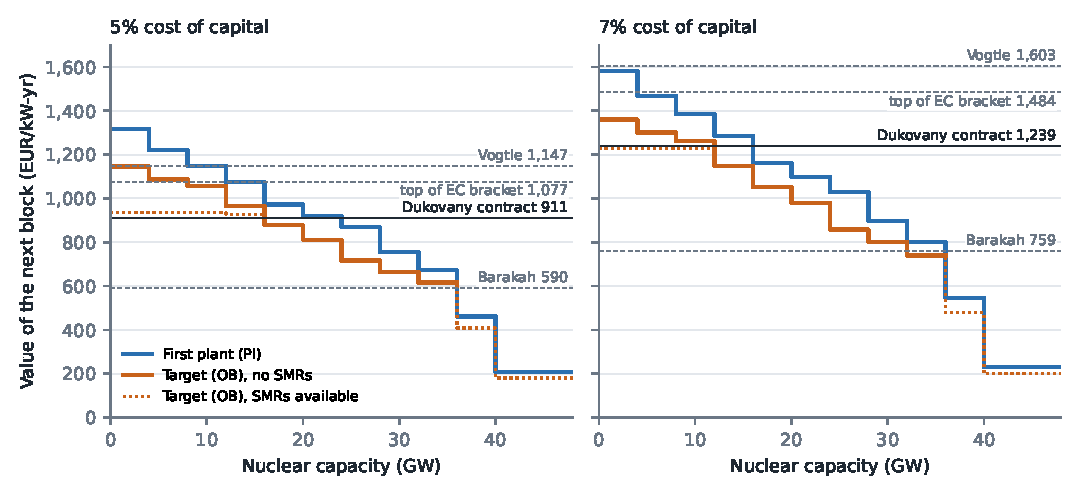
\includegraphics[width=0.84\linewidth]{fig_value_en.pdf}
\caption{Value curve of nuclear capacity: annual fixed cost at which each block of 4\,GW is worth building (8\,GW for the last block), at a 5\% and a 7\% real cost of capital, three-hour step. Horizontal lines: fixN of four cost cases (``Dukovany contract'' is the central case, ``EC bracket'' the Commission's bracket for the overnight cost). Dotted line: OB with SMRs available at target cost, where the fixed capacity is that of large reactors. Source: \texttt{results/v8\_runs.jsonl}.}\label{fig:value}
\end{figure}

\begin{table}[!tb]
\centering\footnotesize
\caption{Marginal value of nuclear capacity by block, EUR/kW-yr, three-hour step. The OB curves without SMRs were computed up to 36\,GW; the two OB curves coincide from 16\,GW at 5\% and from 12\,GW at 7\%.}\label{tab:value}
\begin{tabular}{@{}lrrrrrr@{}}
\toprule
 & \multicolumn{3}{c}{5\% (central fixN 911)} & \multicolumn{3}{c}{7\% (central fixN 1{,}239)}\\
\cmidrule(lr){2-4}\cmidrule(l){5-7}
Block, GW & PI & OB, no SMR & OB, SMR available & PI & OB, no SMR & OB, SMR available\\
\midrule
0--4 & 1{,}318 & 1{,}145 & 934 & 1{,}582 & 1{,}360 & 1{,}231\\
4--8 & 1{,}220 & 1{,}087 & 934 & 1{,}467 & 1{,}301 & 1{,}231\\
8--12 & 1{,}149 & 1{,}058 & 934 & 1{,}387 & 1{,}262 & 1{,}228\\
12--16 & 1{,}074 & 965 & 927 & 1{,}286 & 1{,}148 & 1{,}148\\
16--20 & 973 & 877 & 877 & 1{,}162 & 1{,}054 & 1{,}054\\
20--24 & 921 & 812 & 812 & 1{,}098 & 981 & 981\\
24--28 & 868 & 717 & 717 & 1{,}028 & 858 & 858\\
28--32 & 755 & 663 & 663 & 898 & 802 & 802\\
32--36 & 672 & 616 & 616 & 800 & 740 & 740\\
36--40 & 462 & & 409 & 545 & & 479\\
40--48 & 209 & & 180 & 230 & & 201\\
\bottomrule
\end{tabular}
\end{table}

\subsection{Cost cases read on the curves}\label{sec:casesres}
Table~\ref{tab:casesres} reads the eight cost cases of Table~\ref{tab:cases} on the 5\% curves, and two financing cases in which nuclear alone pays 6\% or 7\%; the 7\% curves and the OB curve with SMRs are in Appendix~\ref{app:curves}. In PI the best capacity on the grid is 24\,GW for the central case and for the 7-year build, 16\,GW for the risk median and for the midpoint of the Commission bracket (12 to 24\,GW within 1\%), and 12\,GW both at the top of the bracket and at the Vogtle cost. The first 4\,GW are worth more than nuclear at the Vogtle cost (1{,}318 against 1{,}147\,EUR/kW-yr), so in PI at 5\% some nuclear is worth building in every cost case examined. This does not hold in OB without SMRs, where the first 4\,GW are worth 1{,}145\,EUR/kW-yr, just below the Vogtle cost: the best capacity is 12\,GW at the midpoint of the bracket (8 to 16\,GW within 1\%), 8\,GW at the top, with a saving of 0.88\,EUR/MWh and every capacity from 0 to 12\,GW within 1\% of the minimum, and zero at the Vogtle cost. At the costs of Barakah and of the Korean budget the best capacity is 36\,GW or more in both PI and OB; these two cases are a floor and a budget, not final costs.

At 7\% (Appendix~\ref{app:curves}) the central case gives 16\,GW in PI and 12\,GW in OB without SMRs on the grid, and the higher cost cases give less: at the midpoint of the bracket 12\,GW in PI (8 to 16 within 1\%) and 4\,GW in OB without SMRs (0 to 8), and little or none above it (Section~\ref{sec:policy}).

\begin{table}[!tb]
\centering\footnotesize
\caption{Cost cases read on the 5\% value curves: best capacity on the 4\,GW grid, range of grid points within 1\% of the minimum cost, and saving against the system without nuclear (EUR/MWh). The OB curve without SMRs ends at 36\,GW. The grid optimum of the central case (24\,GW, saving 13.33) differs from the free optimum of Table~\ref{tab:central} (23.2\,GW, 13.35) only by the grid.}\label{tab:casesres}
\begin{tabular}{@{}lrrrrrrr@{}}
\toprule
 & & \multicolumn{3}{c}{PI} & \multicolumn{3}{c}{OB, no SMR}\\
\cmidrule(lr){3-5}\cmidrule(l){6-8}
Cost case & fixN & Best $N$ & Within 1\% & Saving & Best $N$ & Within 1\% & Saving\\
 & EUR/kW-yr & GW & GW & & GW & GW & \\
\midrule
Saeul and Shin Hanul budget & 426 & 40 & 36--40 & 57.78 & 36 & 36 & 46.04\\
Barakah (floor) & 590 & 36 & 36 & 40.84 & 36 & 32--36 & 29.51\\
Dukovany contract, 7 years & 877 & 24 & 20--28 & 15.64 & 20 & 12--24 & 8.40\\
Dukovany contract, central & 911 & 24 & 16--28 & 13.33 & 16 & 12--20 & 6.85\\
Risk median & 988 & 16 & 12--24 & 9.05 & 12 & 8--16 & 3.64\\
Dukovany, midpoint of the bracket & 991 & 16 & 12--24 & 8.95 & 12 & 8--16 & 3.57\\
Dukovany, top of the bracket & 1{,}077 & 12 & 8--20 & 5.12 & 8 & 0--12 & 0.88\\
Vogtle & 1{,}147 & 12 & 4--16 & 2.76 & 0 & 0--8 & 0.00\\
\midrule
Contract cost, nuclear at 6\%$^{a}$ & 1{,}064 & 16 & 8--20 & 5.65 & 8 & 4--12 & 1.16\\
Contract cost, nuclear at 7\%$^{a}$ & 1{,}235 & 4 & 0--12 & 0.93 & 0 & 0--4 & 0.00\\
\bottomrule
\multicolumn{8}{@{}p{\linewidth}@{}}{$^{a}$ Nuclear financed at 6\% or 7\%, every other technology and the grid charge at 5\%; SMRs at 7\% (1{,}226\,EUR/kW-yr with the grid charge at 5\%) would not enter either.}
\end{tabular}
\end{table}

\subsection{A flat optimum}\label{sec:flat}
Figure~\ref{fig:cost} shows the system cost against nuclear capacity at the central cost and 5\%. In PI the cost is 115.245\,EUR/MWh at 16\,GW, 114.436 at 24\,GW and 114.913 at 28\,GW: a change of 12\,GW in nuclear capacity changes the system cost by at most 0.81\,EUR/MWh (our calculation), less than 1\%. The range of grid points within 1\% of the minimum is 16--28\,GW in PI at 5\%, 12--20\,GW in PI at 7\%, 12--20\,GW in OB at 5\% and 4--16\,GW in OB at 7\%; on the OB curves where SMRs fill the gap left by large reactors, and N counts large reactors only, the range is 0--20\,GW at 5\% and 0--12\,GW at 7\%. Around the optimum, therefore, small changes in any cost move the optimal capacity by several GW while the system cost barely changes. Far from it the cost is not flat: in PI at 5\% a system with 36\,GW costs 4.3\% more than the optimum.

\begin{figure}[!tb]
\centering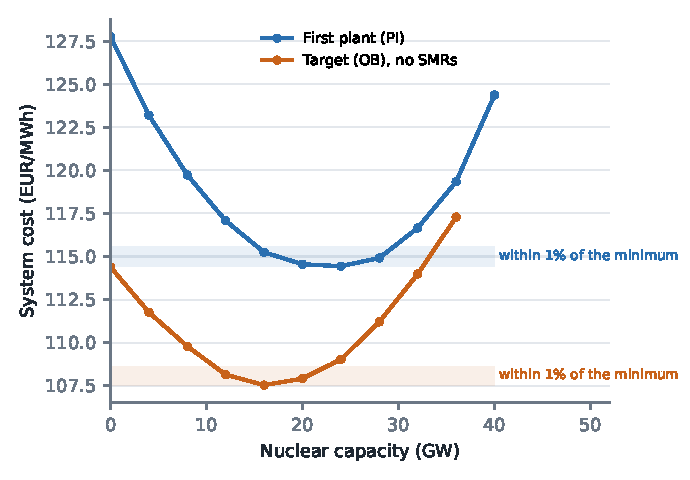
\includegraphics[width=0.52\linewidth]{fig_cost_en.pdf}
\caption{System cost against nuclear capacity at the central nuclear cost (fixN 911) and a 5\% cost of capital, three-hour step, with the band within 1\% of the minimum. Source: \texttt{results/v8\_runs.jsonl}.}\label{fig:cost}
\end{figure}

\subsection{Systems with and without nuclear}\label{sec:systems}
Table~\ref{tab:systems} compares the central systems at 5\%. In PI the system without nuclear needs 193\,GW of PV against 76, with every ground-mounted and agrivoltaic block at its cap, and two of the three industrial-roof blocks, and 59.6\,GW of onshore wind against 33.4, every block except the worst (10\,GW at 1{,}200 hours; 69.6\,GW are available). It needs 281\,GWh of batteries against 129 and 14.8\,TWh of hydrogen storage against 2.1, and it swaps 27.7\,TWh a year with the neighbours in each direction against 17.7. In cost terms, without nuclear PV costs 56.19\,EUR/MWh against 16.97, batteries 17.00 against 7.77 and hydrogen 11.22 against 4.98, and the system pays 4.57\,EUR/MWh of second grid charge above the 137\,GW threshold; the system with nuclear pays 65.43\,EUR/MWh for nuclear, which runs at a load factor of 87.5\%. In OB the system with nuclear relies on 10\,GW of CSP, 214\,GWh of compressed air and 310\,GWh of 100-hour storage next to 15.7\,GW of nuclear; without nuclear it adds PV (161\,GW against 85), batteries, hydrogen storage and 100-hour storage (632\,GWh). CSP is at its ceiling of 10\,GW in both OB systems; the ceiling is our assumption.

\begin{table}[!tb]
\centering\footnotesize
\caption{Central systems at 5\%, three-hour step. PV and onshore wind include the existing plants kept in the model. Hydrogen store in TWh (our conversion from GWh). Swap: energy exchanged with neighbours in each direction.}\label{tab:systems}
\begin{adjustbox}{max width=\linewidth}
\begin{tabular}{@{}lrrrrrrrrrrrr@{}}
\toprule
System & PV & Onshore & Offshore & Nuclear & CSP & Batteries & Hydrogen & Compr. & 100-hour & Intercon- & Swap & Nuclear\\
 & & wind & wind & & & & store & air & storage & nection & & load factor\\
 & GW & GW & GW & GW & GW & GWh & TWh & GWh & GWh & GW & TWh/yr & \%\\
\midrule
PI with nuclear & 76 & 33.4 & 0.0 & 23.2 & 0.0 & 129 & 2.1 & 0 & off & 13.9 & 17.7 & 87.5\\
PI without & 193 & 59.6 & 2.6 & 0.0 & 0.0 & 281 & 14.8 & 0 & off & 18.9 & 27.7 & \\
OB with nuclear & 85 & 44.6 & 0.0 & 15.7 & 10.0 & 13 & 4.1 & 214 & 310 & 13.6 & 20.2 & 89.1\\
OB without & 161 & 59.6 & 2.0 & 0.0 & 10.0 & 152 & 8.7 & 80 & 632 & 18.1 & 29.8 & \\
\bottomrule
\end{tabular}
\end{adjustbox}
\end{table}

\subsection{Variants}\label{sec:variants}
Table~\ref{tab:variants} gives the free optimum at 5\% when assumptions change. Nine rows change one assumption (the MACSE battery row changes the product, so price and duration together); two rows, marked as bundles, change several at once.

\emph{Trade.} If exports earn nothing the optimum is 25.4\,GW in PI and 18.3\,GW in OB; if they earn the import price it is 18.0 and 14.1\,GW. Allowing net exports changes little. Allowing net imports of up to 10\% of demand leaves the PI optimum at 23.4\,GW and lowers the OB optimum to 12.6\,GW. Choosing the critical weeks by low PV and wind output, as in the previous version, gives 18.2 and 14.5\,GW.

The trade rule of the previous version gives 11.9\,GW in PI and 7.2\,GW in OB, about half the central values, but it is a bundle of five changes: 38\% of the import capacity is available and counts as firm in the critical weeks; those weeks are chosen by low PV and wind output; imports cost 1.17 times the price in those weeks; nothing is exported; and there is no annual balance. Under it the model builds all 7.33\,GW of new lines and Italy imports 52 to 71\,TWh a year net. Taken one at a time: 10\% net imports give 23.4 and 12.6\,GW; weeks chosen by low PV and wind 18.2 and 14.5\,GW; the 38\% foreign credit alone, with the annual balance kept, 17.9 and 14.1\,GW. The credit is the largest single change in PI, about half of the drop, but only 1.6\,GW in OB. No single change explains the halving, which comes from the combination with the missing annual balance (Section~\ref{sec:dependence}).

\emph{Costs and weather.} With batteries at the MACSE award price (about 95\,EUR/kWh for systems of about 6.6 hours, against our 168.6 for 4-hour systems; not the same product), which also sets their duration at 6.6 hours, the optimum is 18.1 and 14.0\,GW: it stays at or above about 15\,GW in PI and near it in OB, so the recommendation of about 15\,GW does not change. Batteries move energy by hours, from day to evening, and that is already cheap; what nuclear replaces is firm energy in the winter weeks with little sun and wind, which without nuclear comes from hydrogen. Hydrogen, not batteries, is the bottleneck, and it is costed optimistically (Table~\ref{tab:limits}). With eight weather years, the four central ones and the four worst, it is 27.1\,GW in PI and 15.5\,GW in OB (about unchanged from 15.7); the added years reuse the load of 2016--2019, so there load and weather are not of the same year. A 7-year build gives 26.7 and 18.2\,GW. With nuclear at the top of the Commission bracket the optimum is 14.0\,GW in PI and 14.4\,GW in OB: OB has more nuclear than PI here, because its SMRs are at target cost and all 14.4\,GW are SMRs; with large reactors alone OB has 8\,GW (Table~\ref{tab:casesres}). The last row is the second bundle: the nuclear inputs of the previous version (8{,}540\,EUR/kW, 7 years, 80-year life, O\&M of 32\,EUR/MWh, availability 92\%; fixN 670) with the present costs of the other technologies.

With the annual balance and no foreign capacity in the critical weeks, the optimum is between 14.0 and 27.1\,GW in PI and between 14.0 and 18.3\,GW in OB in every variant except the bundle with the previous nuclear inputs (33.6 and 28.4\,GW). The variants that drop these rules give less: 12.6\,GW in OB with net imports up to 10\%, and 11.9 and 7.2\,GW with the trade rule of the previous version. Among the system rules the trade rule moves the result most; the cost of nuclear moves it more, since the cost cases span 0 to 40\,GW.

\begin{table}[!tb]
\centering\footnotesize
\caption{Variants at 5\%, free optimum, three-hour step. Each row changes one assumption, except the two bundles, which change several; the MACSE battery row changes the product, so price and duration together. Nuclear in GW (SMRs included); cost of the system with nuclear and saving against the system without nuclear under the same assumptions, EUR/MWh.}\label{tab:variants}
\begin{tabular}{@{}P{7.0cm}rrrrrr@{}}
\toprule
 & \multicolumn{3}{c}{PI} & \multicolumn{3}{c}{OB}\\
\cmidrule(lr){2-4}\cmidrule(l){5-7}
Variant & Nuclear & Cost & Saving & Nuclear & Cost & Saving\\
\midrule
Central & 23.2 & 114.42 & 13.35 & 15.7 & 107.53 & 6.86\\
Exports earn nothing & 25.4 & 117.20 & 15.26 & 18.3 & 110.50 & 8.58\\
Exports earn the import price (115.94\,EUR/MWh) & 18.0 & 111.10 & 11.86 & 14.1 & 103.71 & 5.56\\
Net imports allowed up to 10\% of demand & 23.4 & 114.11 & 11.81 & 12.6 & 107.12 & 4.09\\
Net exports allowed & 22.8 & 114.09 & 13.68 & 15.8 & 107.52 & 6.87\\
Critical weeks chosen by low PV and wind output & 18.2 & 113.64 & 10.45 & 14.5 & 107.03 & 6.50\\
Bundle: trade rule of the previous version (five changes, see text) & 11.9 & 109.99 & 5.96 & 7.2 & 103.38 & 2.14\\
Batteries at the MACSE award price, 6.6 hours & 18.1 & 108.92 & 11.38 & 14.0 & 105.09 & 4.99\\
Eight weather years (2016--2019, 1994, 1998, 2014, 2015) & 27.1 & 118.62 & 17.49 & 15.5 & 110.71 & 7.97\\
Nuclear built in 7 years & 26.7 & 112.02 & 15.75 & 18.2 & 105.90 & 8.48\\
Nuclear at the top of the Commission bracket (12{,}700\,EUR/kW) & 14.0 & 122.56 & 5.21 & 14.4$^{a}$ & 108.50 & 5.89\\
Bundle: nuclear inputs of the previous version (fixN 670) & 33.6 & 95.46 & 32.31 & 28.4 & 92.77 & 21.62\\
\bottomrule
\multicolumn{7}{@{}l}{$^{a}$ All SMRs at target cost.}
\end{tabular}
\end{table}

\subsection{Time step}\label{sec:step}
The same model at a six-hour step gives 21.7\,GW in PI and 13.7\,GW in OB at 5\%, against 23.2 and 15.7\,GW at three hours: the finer step raises the optimum by 1.6\,GW in PI (23.22 against 21.66) and 1.9\,GW in OB (15.65 against 13.73). The adequacy requirement is the same at both steps, so the difference does not come from the reserve. Hourly data were not rebuilt: the direction of the effect is known from the sequence of 12-, 6- and 3-hour steps (nuclear at 17.4, 21.7 and 23.2\,GW in PI and 6.0, 13.7 and 15.7\,GW in OB; the 12-hour runs are the repository's smoke tests, \texttt{tests/expected\_smoke\_h12.jsonl}), its size at one hour is not, so the three-hour results may still understate nuclear slightly. Only three-hour results are compared with each other in this paper.

\subsection{Small modular reactors in the target case}\label{sec:smr}
At their target cost SMRs are near-perfect substitutes of large reactors at the central cost: 934 against 911\,EUR/kW-yr at 5\%, and 1{,}231 against 1{,}239 at 7\%. The order changes with the rate because the 5-year build of SMRs, against 9 years, saves more interest during construction at 7\%; the 5 years is the vendor's schedule for the first Darlington unit, not an observed build, and with 7 years the advantage would disappear. The model therefore builds only large reactors at 5\% (15.7\,GW) and only SMRs at 7\% (11.1\,GW), but the choice is worth little: at 7\% the system with 11.0\,GW of large reactors and no SMRs costs 0.27\,EUR/MWh more (our calculation).

The OB curve with SMRs available (dotted in Fig.~\ref{fig:value}) shows the substitution. When large reactors are fixed below the optimum, SMRs fill the gap, so a further block of large reactors is worth only the cost of the SMRs it displaces: 934, 934 and 927\,EUR/kW-yr for the blocks between 4 and 16\,GW at 5\%, and 1{,}231 and 1{,}228 for the blocks between 4 and 12\,GW at 7\%. Its point at zero is the system with SMRs only (14.4\,GW at 5\%, 11.1\,GW at 7\%), which does not depend on the cost of large reactors, so the first block is also worth the SMRs it displaces (934 at 5\%, 1{,}231 at 7\%). The value of nuclear as a whole is the curve without SMRs; the two curves coincide from 16\,GW at 5\% and from 12\,GW at 7\%, where no SMR is built.

With SMRs at target cost, therefore, the system is almost insensitive to the cost of large reactors above about 934\,EUR/kW-yr. This rests on a target, the cost of the four-unit Darlington programme with the operating cost of large reactors as a proxy; at the first-plant cost (1{,}264\,EUR/kW-yr at 5\%) SMRs play no material role.
\FloatBarrier

\section{Discussion}\label{sec:discussion}

\subsection{The import-dependence choice}\label{sec:dependence}
Among the system rules, the trade rule has the largest effect (Table~\ref{tab:variants}). The looser trade rule about halves nuclear, to 11.9\,GW in PI and 7.2\,GW in OB, and the saving from nuclear falls from 13.35 to 5.96\,EUR/MWh in PI and from 6.86 to 2.14 in OB. That rule is a bundle of five changes (Section~\ref{sec:variants}), and the halving cannot be attributed to one of them: it comes from foreign plants available in the critical weeks together with no annual balance, so that imports become a firm source all year. Of the single changes we have, a net-import allowance of 10\% of demand matters little in PI, where the optimum goes from 23.2 to 23.4\,GW, and matters in OB, where it goes from 15.7 to 12.6\,GW and the saving from 6.86 to 4.09\,EUR/MWh; the allowance lowers the cost of the PI system by 0.31\,EUR/MWh with nuclear (from 114.42 to 114.11) and by 1.85 without it (from 127.77 to 125.92).

The price of the central rule is the difference in system cost against the looser trade rule, at 5\% and in EUR/MWh. With nuclear the system costs 114.42 against 109.99 in PI (4.44 more, EUR\,1.6 billion a year) and 107.53 against 103.38 in OB (4.15 more, EUR\,1.5 billion). Without nuclear it costs 127.77 against 115.95 in PI (11.82 more, EUR\,4.2 billion) and 114.39 against 105.52 in OB (8.87 more, EUR\,3.2 billion). Under the looser rule Italy imports 52.0\,TWh a year (PI with nuclear), 57.7 (PI without), 56.0 (OB with) and 70.7 (OB without) and exports nothing; in 2025 it imported 55.2\,TWh and exported 7.4, a net 47.8\,TWh \citep{GME2025}. The looser rule is therefore about today's dependence, and the central case of this paper is a choice to end it. So the comparison that matters is not between today's import share and that of 2040, but between a system that does not rely on its neighbours in the critical weeks and one that does.

The central rule raises the nuclear optimum: counting 38\% of foreign capacity as firm in the critical weeks, with the annual balance kept, gives 17.9 instead of 23.2\,GW in PI and 14.1 instead of 15.7\,GW in OB. It is not a bias but the planning standard: a plan that counts on neighbours' capacity in those weeks counts on their plants, largely French and Swiss nuclear, as the evidence below shows. The critical weeks all fall between November and February (2016: January, November, December; 2017 and 2018: January, February, November; 2019: January, November, December). Weeks of this kind are not rare: over 38 weather years and 33 countries, Europe has on average about four periods a year of at least a week with combined wind and solar output below 75\% of the mean, and in a perfectly interconnected Europe the longest, in the winter of 1996/97, lasted 55 days \citep{KittelSchill2024}; we found no estimate specific to Italy. The rule that ranks weeks by lowest PV and wind output (which picks an August week) shares only 4 of the 12 weeks. In 2024, 85\% of Italy's imports came from Switzerland (43\%) and France (42\%) \citep{Sole2024imports}. In winter France has its own peak and its firm capacity is nuclear; Switzerland was a net importer on almost every day of winter 2025/26, with the Gösgen nuclear plant offline \citep{Economiesuisse2025}; France was a net importer in 2022, when it had to stop reactors \citep{BdF2023}. The European Resource Adequacy Assessment 2025 of ENTSO-E shows rising adequacy risks [VERIFY: ENTSO-E, ERAA 2025]; Terna's adequacy report models the neighbouring countries as subject to the same critical conditions as Italy [VERIFY: Terna, Rapporto Adeguatezza Italia 2024, modelling of neighbours]; and the 4.4\,GW of foreign capacity in the Italian capacity market is admitted capacity, not a guaranteed import [VERIFY: source of the 4.4\,GW, Italian capacity market 2025]. Relying on imports in those weeks therefore means relying largely on foreign nuclear plants when they are needed at home, and a system without Italian nuclear built that way imports nuclear. Self-sufficiency costs more without nuclear for the same reason: the system without nuclear leans more on its neighbours. How much foreign capacity will be free in winter in 2040 cannot be known or guaranteed, and that is why the central case does not count on it: a national plan cannot rest on the hope that other countries will have spare energy and sell it in the weeks when everyone needs it. The rule is therefore the planning standard, not a limit, and it is not listed in Table~\ref{tab:limits}.

The price earned by exports is the remaining uncertainty in the central rule. It is an annual average of the French price, while the surplus of a system with much solar occurs when the neighbours also have a surplus. Between exports that earn nothing and exports that earn the import price the PI optimum goes from 25.4 to 18.0\,GW. The average price favours the system that exports more, the one without nuclear (27.7 against 17.7\,TWh a year in PI), so this simplification works against nuclear.


\subsection{Why other studies reach different conclusions}\label{sec:others}
Other studies reach other results for reasons that can be identified: a different cost or cost of capital for nuclear, a coarser treatment of time and weather, imports counted as available in winter, net-zero rather than zero direct emissions, caps on nuclear, and cost projections. On the last point, most of the studies below project costs to 2040 or 2050 for some or all technologies; we use today's contract or plant price for every technology, because the decision is taken now (Section~\ref{sec:rule}). For each study we give what it finds, the assumption that drives the difference and the direction of that assumption on nuclear.

\paragraph{Cost per MWh.} The cost per MWh depends on the hours assumed. In the IEA tables, European nuclear in 2030 has a construction cost of 5{,}100\,USD/kW and a load factor of 75\% \citep[Annex~B, Tables B.4a and B.4b]{IEA2024WEO}. The world fleet ran at 83\% in 2024 \citep{WNAPerformance2025} and the US fleet at 92\% \citep{EIA2025TIE}. At the fixN of our central case, 918\,EUR/kW-yr, a reactor running at 75\% costs about 152\,EUR/MWh, against 132\,EUR/MWh at the 87.5\% of the PI optimum: 15\% more (our calculation). For PV the same tables assume a load factor of 14\% \citep[Table B.4a]{IEA2024WEO}, about 1{,}226 hours a year (our calculation, $0.14 \times 8{,}760$), while the Italian fleet ran 1{,}117 hours in 2025 \citep{GSEPV2025}: at the same plant cost the Italian MWh costs about 10\% more (our calculation).

\citet{Lazard2026} reports 175--255\,USD/MWh for new nuclear in the United States, from the public cost estimates of Vogtle 3 and 4, 12{,}300--17{,}570\,USD/kW, with an after-tax cost of capital of 7.7\%; the high end is unit~3 and the low end unit~4. This is a first-of-a-kind American cost at a higher cost of capital: our Vogtle case (13{,}400\,EUR/kW, 10 years) costs about 162\,EUR/MWh at 5\% and a load factor of 87.5\% (our calculation), and it is a cost case on the curve, not the central case. \citet{FraunhoferEN2024} reports 136--490\,EUR/MWh for nuclear in Germany, with 4{,}300--6{,}300 full-load hours today and 2{,}000--4{,}000 by 2045, 6{,}000--16{,}000\,EUR/kW and a real cost of capital of 7.8\%. The hours drive the range: at our central fixN of 918\,EUR/kW-yr a plant that runs 4{,}300 hours costs about 226\,EUR/MWh and one that runs 2{,}000 hours about 471, against 132\,EUR/MWh at the 7{,}670 hours of the PI optimum (our calculation). The same report gives 6.0--22.5\,ct/kWh for PV with batteries: 6.0--10.8 for large ground-mounted plants and 9.1--22.5 for small roofs. These are plants that shift part of their own output by a few hours, not systems that meet demand in every hour.

\citet{Lund2026} find that in Denmark the cost of renewables, system cost included, is ``significantly lower'' than that of nuclear; the figure of 53\% cheaper is a press headline and is not in the paper. Their main scenario uses an equivalent nuclear capital cost of 10{,}000\,EUR/kW at a 5\% discount rate, which represents the IEA's 6{,}500\,EUR/kW at 8\%. That cost is close to our 10{,}300 at 5\%, so the difference comes from the system modelled and the method, which we have not examined further. A dossier of Banca d'Italia, as reported by \citet{QEBankitalia2025}, gives 188--991\,USD/MWh for water-cooled reactors; the article cites, just before the range, a study of 19 designs of small, advanced and micro reactors \citep{Steigerwald2023}, which suggests that the range refers to those designs and not to large reactors. The dossier itself was not read. The scenarios of \citet{ItaliaSolare2026} assume 11{,}000\,EUR/kW for nuclear in 2040 and 9{,}000 in 2050, with a 5\% cost of capital for every technology, allow investment in nuclear only from 2040 and report no nuclear capacity. Their 2040 value is 7\% above our central cost (our calculation) and lies between it and the midpoint of the Commission bracket.

\paragraph{Firm resources and system cost.} \citet{Sepulveda2018} find that firm low-carbon resources (nuclear, gas with capture and bioenergy) lower the cost of fully decarbonised power systems by 10--62\% (abstract); expressed as the increase without them, this is 11--163\% (our conversion). For the OECD Nuclear Energy Agency the system costs of variable renewables rise from 8\,USD/MWh at a 10\% share to 50\,USD/MWh at 75\% \citep{NEA2019}. In our central results the system without nuclear costs 11.7\% more than the one with nuclear in PI (127.77 against 114.42\,EUR/MWh) and 6.4\% more in OB (114.39 against 107.53; our calculation): at the bottom of the range of \citeauthor{Sepulveda2018} in PI and below it in OB. In money the savings, 13.35 and 6.86\,EUR/MWh, are about 15 and 8\,USD/MWh at 1.1188\,USD per euro (our conversion), in the low part of the range of the Agency, although the two quantities are not the same and the comparison is one of order of magnitude only. The saving is modest because our system without nuclear keeps other firm sources: hydro, geothermal, bioenergy, hydrogen turbines, and the swap with the neighbours outside the critical weeks. How much of it each one provides, and the saving with no imports at all, need runs still to do (Section~\ref{sec:variants}).

\paragraph{Italian studies with nuclear.} \citet{Mastrantuono2026} use TEMOA-Italy, with 20 regions and 96 time slices a year (four seasons of 24 hours), no weather years and no adequacy check. Imports are modelled at average capacities and prices; hydrogen is not modelled in the power sector, and the only storage is batteries and pumped hydro. Nuclear enters from 2040 and is capped at 1.6, 3.2 and 8.0\,GWe in 2040, 2045 and 2050; its overnight cost is 4{,}000\,USD/kW in 2022 dollars, contingency included (about 3{,}575\,EUR/kW at 1.1188, without inflation; our conversion), with a 10-year build and hurdle rates of 6--10\%, while totals are discounted at 5\%. Nuclear is built in 23 of 27 scenarios; in the scenarios with stable costs the 8\,GWe cap is always reached, and the saving is up to almost EUR\,8 billion in present value. Nuclear lowers storage by up to 42\%, curtailment by about 35\% and land use by about 25\%; on imports the paper gives both ``up to 22\%'' and ``nearly 50\%''. Because the cap binds, 8\,GWe is a lower bound of the economic amount, not an optimum. The lower cost of nuclear pushes towards more nuclear than ours; the higher hurdle rates, the time slices without weather years or critical weeks, and imports without a test in scarce periods push towards less; the absence of hydrogen works both ways. At their cost and build time fixN is 478\,EUR/kW-yr at 5\% and 603 at 7\% (our calculation), and on our value curves the best capacity is 36\,GW in PI and at least 36\,GW in OB, the end of the computed OB curve [RUN: free optimum at 3{,}575\,EUR/kW with a 10-year build, PI and OB at 5\% and 7\%]: the cap would bind in our model as well.

The preprint of \citet{CataniaSSRN}, from the Politecnico di Milano and the Università dell'Insubria, could not be read, and its nuclear figures could not be checked. Its model, FENICE, is public \citep{FENICE}, and the open companion paper of the same group \citep{Catania2026} describes it: 24 typical days per year, 20 regions, carbon neutrality by 2050 with direct air capture and CO$_2$ storage up to 16\,Mt a year, electricity imports up to 40\,TWh a year with no test of their availability in critical periods, nuclear allowed only from 2045, and a 0\% discount rate in the base case of that paper. The input file of the repository, written for the companion study, projects costs with learning, for example PV from 752 to 287\,EUR/kW and large nuclear from 6{,}423 to 5{,}537\,EUR/kW between 2025 and 2055. Typical days without critical weeks, net zero with direct air capture, imports without a test in winter, late entry of nuclear and falling costs for PV, batteries and hydrogen all push towards less nuclear; a 0\% discount rate pushes towards more. The net-zero rules in our model are a run still to do [RUN: net-zero mode with gas with capture and direct air capture, PI and OB at 5\%]. At 5{,}500\,EUR/kW and 8 years (fixN 590 at 5\%, the Barakah case) our value curve already gives 36\,GW in PI, the top of the computed range [RUN: free optimum at 5{,}500\,EUR/kW with an 8-year build, PI and OB at 5\%].

\citet{Stevanato2026}, a preprint not yet peer reviewed, plan the system with one average day and one node, then test the plan hour by hour on weather years that include a two-week episode of low wind and sun, where only batteries can be added. In the net-zero case led by renewables the batteries grow from 473 to 26{,}107\,GWh and the system cost from 699 to 1{,}866 billion euros in that episode (1{,}393 billion in the typical year); with SMRs at low cost the batteries stay at 161--183\,GWh and the correction is within 10 billion euros. Their SMRs, uncapped from 2036 and partly used for heat, reach 20.3\,GWe in 2050 at 4{,}250\,EUR/kWe and 9.09\,GWe at 8{,}500, with a 3\% social discount rate. The 26\,TWh of batteries measure how badly a plan built on one average day fails when only batteries can respond, not the least-cost firm mix; the result supports planning on critical weeks with the real weather sequence, as we do. Their 3\% rate and the value of heat push towards more nuclear, and net zero with 3.6--3.8\,GW of gas with capture towards less. \citet{DiBella2025} show for 2030 that resilience to extreme weather years needs 5--8\,GW more PV; nuclear is excluded in their model for political reasons, so the study supports the use of several weather years but does not bear on nuclear.

The 2024 national energy and climate plan expects about 8\,GW of nuclear by 2050, 16\,GW in an ambitious option, with a climate cost EUR\,17 billion lower than without nuclear \citep{WNNPNIEC2024}; the shares quoted with it (``more than 10\%'' and ``over 20--22\%'') do not say whether they are of capacity or of electricity. These are policy scenarios, not optima. On our 5\% curves with a 9-year build, 8--16\,GW corresponds to fixN of 973--1{,}220\,EUR/kW-yr in PI and 877--1{,}087 in OB, that is construction costs of about 11{,}100--14{,}900 and 9{,}700--12{,}900\,EUR/kW (our reading: the ends are the values of the blocks on either side). The contract cost, 10{,}300\,EUR/kW, lies below the PI range and inside the OB range: building at the Dukovany contract makes at least the plan's 16\,GW economic at 5\%, in PI and in OB. \citet{Battaglia2025} compare the two scenarios of the plan with EnergyPLAN, an hourly model: in the scenario with nuclear, capped at 8\,GW by 2050, emissions fall by about 7\,Mt of CO$_2$ a year (abstract read). The cap is set outside the model, so the result cannot be compared with our value curve.

\paragraph{Studies without nuclear.} \citet{Pastore2025a} describe a fully renewable Italy in 2050 with an hourly model, with a potential of 115.4\,GW of onshore and 55.7\,GW of offshore wind, all of it installed in most scenarios. Our onshore supply is 69.6\,GW, below the 96.9\,GW of the medium-tolerance scenario of \citet{Price2026}, so their result rests on sites beyond our curve. A companion paper \citep{Pastore2025b} gives 44\,EUR/MWh for electricity plus 8.5\,EUR/MWh of storage, 52.5 in all, without hydrogen; it uses 2050 costs, including 1.64\,MEUR/MW for offshore wind, and 3{,}092\,GWh of hydrogen storage. At its own 2050 cost for hydrogen tanks, 0.22\,MEUR/MWh, that storage would cost about 680 billion euros (our calculation), 2.7 times the 250 billion the paper gives for the whole hydrogen chain; the paper does not explain the difference. The same group finds 4.85--5.91\,MEUR/MW for floating offshore wind in the Mediterranean in the short term and 4.13 in the medium term \citep{Vespasiano2026}, 2.5 times the 2050 value used for Italy (our ratio). Wind beyond our curve, 2050 costs and the unclear cost of hydrogen storage all lower the cost of the system without nuclear. In our model floating offshore wind costs 4{,}750\,EUR/kW, close to that short-term value, and the PI system without nuclear builds 2.6\,GW of it.

\citet{Lombardi2020} find near-optimal Italian systems without nuclear with an hourly model of 20 regions and one weather year. In the cost-optimal case electrolysis and methanation with carbon from direct air capture make synthetic methane, stored in the existing gas network for long periods, and of today's gas turbines the near-optimal alternatives rarely keep more than about 20\% of the capacity and never more than 60\%; under adverse weather more renewables and batteries are needed. The cost-optimal case adds 144.5\,GW of PV, 59.6\,GW of onshore and 17.6\,GW of offshore wind, with 11.7\,GW of existing combined-cycle gas plants, 7.0\,GW of electrolysis (as hydrogen) and 5.6\,GW of methanation (as methane). The paper does not report the annual volume of synthetic methane. Its own capacities set a ceiling: 5.6\,GW of methanation at full load all year give about 49\,TWh, about 4.6 billion m$^3$ a year; and every 10 points of load factor on the 11.7\,GW of combined cycles, at 55\% efficiency, need about 1.76 billion m$^3$ a year (our calculation, at 10.57\,kWh per m$^3$). This chain does not exist at industrial scale; the biomethane injected into the Italian grid today is about 0.57 billion m$^3$ a year, from 115 plants \citep{QEBiomethane2024}: the synthetic-methane ceiling is about 8 times that, and every 10 points of load factor about 3 times; on today's biomethane alone those plants would run at a load factor of 3.2\% (our calculation). \citet{Franzmann2026} obtain 91.6\,EUR/MWh for a fully renewable Europe in 2050, over 20 weather years, with 1{,}116\,GW of electrolysers and 501\,GW of hydrogen back-up plants; hydrogen infrastructure is 22\% of the cost, the only sensitivity is on the value of lost load, nuclear is not considered, and the authors note that constraints on transport capacity could change the results. In both studies, as in our system without nuclear, firm supply in winter rests on a hydrogen or synthetic-fuel chain without market prices.

\paragraph{Net zero instead of zero emissions.} Models with a net-zero target can cover the winter with gas plants with carbon capture and offset the rest with direct air capture. No gas plant with capture is yet in operation. The first, Net Zero Teesside in the United Kingdom, up to 742\,MW and about 2\,Mt of CO$_2$ a year, is expected to start in 2028, and its contract terms are not public \citep{NZT2026}. The only power plant with capture and years of operation, the coal-fired Boundary Dam~3 in Canada, captured 57\% of its CO$_2$ to the end of 2023 against the 90\% promised, and capture was available in about 80\% of the hours \citep{IEEFA2024}. In Italy Ravenna CCS plans to store 4\,Mt of CO$_2$ a year by 2030 from industrial emitters \citep{Eni2026}. Capture adds about 37--75\,GBP per MWh of electricity, the low end at about 110\,GBP per tonne, the most optimistic estimate, and other estimates are up to twice as high \citep{Goodall2025}. At the 2025 Italian gas price of 38.53\,EUR/MWh \citep{GME2025}, the fuel alone of a combined cycle with capture at 50\% efficiency costs about 77\,EUR per MWh of electricity (our calculation). Direct air capture is further away: the largest plant, Mammoth in Iceland, removed 675\,t of CO$_2$ in the first half of 2026, against a nameplate of up to 36{,}000\,t a year \citep{EnergyConnects2026}. A result with little nuclear that depends on these technologies holds only if they reach the cost and performance assumed; Teesside will show part of it after 2028.

\subsection{Construction cost and time}\label{sec:construction}
Three variables that policy can influence set the annual fixed cost of nuclear: construction cost, build time and cost of capital (Section~\ref{sec:policy}). Construction cost falls with a series of one design. The World Nuclear Association reports an expected cost of 2{,}700\,USD/kWe for Saeul 3 and 4 and 2{,}487\,USD/kWe for a series unit in Korea \citep{WNAKorea,WNAEconomics}; the Barakah contract, first fuel included, is about 3{,}790\,USD/kW for four units of 1{,}345\,MWe net (our calculation from \citealp{WNAuae}). The Dukovany contract with the same vendor is 8{,}446\,EUR/kW net for construction alone. The Western first-of-a-kind builds are higher and slower. Flamanville~3 started operation 17 years after construction began and cost a little over EUR\,13 billion against an initial budget of 3 billion \citep{IlPostFlamanville}; Hinkley Point~C will start its first reactor in 2030, almost 13 years after construction began, at GBP\,35 billion in 2015 prices \citep{GuardianHPC2026}. These are first projects of their design in their country. Across the world, the median construction time of reactors started since 1990 is 5.7 years and 89\% took less than ten years; over all reactors the median is 6.3 years and 83\% took less than ten \citep{Ritchie2023}. Japan builds in less than 5 years, South Korea and China in less than 6 \citep{Ritchie2023}. Our central 9 years, from the Czech financial model, is above that median.

The causes of delay are documented. For Flamanville the Folz report of 2019 points to faulty welds, underestimated complexity, engineering incomplete when construction started, weak project governance and skills lost after years without new plants; it also cites the change in the rules on pressure equipment \citep{Folz2019}. That industrial causes weigh more than regulatory ones is our reading. In the United States of the 1970s and 1980s rules changed during construction weighed instead: reactors under construction during the Three Mile Island accident had median costs 2.8 times and median build times 2.2 times those completed before \citep{Pielke2026}. What makes a programme build well is known in kind: one standard design built in series, engineering completed before construction starts, and rules fixed before the start. For this reason the central case is a plant built well, and the first-of-a-kind builds are cost cases on the curve (Section~\ref{sec:nuclear}). At the contract cost, 7 instead of 9 years raises the optimum to 26.7\,GW in PI and 18.2\,GW in OB. Fifteen years, as in the risk median, gives fixN 1{,}037\,EUR/kW-yr at 5\%, and the best capacity on the curves is 16\,GW in PI and 12\,GW in OB; at 7\% (fixN 1{,}510) it is 4\,GW in PI and none in OB (our reading).

Small modular reactors do not lower these values. According to a literature review of 2024 they cost on average about 41\% more per kW than large reactors, and a first unit up to twice as much according to the IEA \citep{HSFSMR2026}. In our inputs the four-unit Darlington programme costs 14\% more per kW than the Dukovany contract and the first unit 67\% more (our calculation). The 5{,}000\,EUR/kW quoted for SMRs by the national platform for sustainable nuclear (PNNS) [VERIFY: QualEnergia, 16 October 2026] is therefore far from existing contracts; the even lower press estimate for an Italian SMR, 3{,}500--5{,}500\,EUR/kW, is not used as an input (Section~\ref{sec:nuclear}).

\subsection{Deployment rate and siting}\label{sec:deployment}
About 15\,GW is about 15 APR1000 units of 976\,MW net, and 23.2\,GW about 24. With a first unit around 2036 (Dukovany plans works from 2029 and the first grid connection in December 2036; \citealp{ECDukovany2026}), 15 units by 2050 need about one unit, or 1\,GW, a year. Korea connected seven reactors to the grid between 1983 and 1989, with eight under construction in the early 1980s \citep{WNAKorea}: about one a year. The required pace is similar, in a country that restarts without a complete supply chain. France connected 52 reactors to the grid between 1977 and 1990, 54.4\,GW net, on average 3.9\,GW a year, with peaks of 8 reactors in 1981 and 7.4\,GW in 1986 (our count from the IAEA tables, with the Superph\'enix fast reactor and with today's net ratings, not those at connection; \citealp{IAEACNPPFrance}): the pace required of Italy would be about 26\% of the French average of that time (our calculation). The model does not compute a transition, but the value curve gives the cost of a fleet that stays smaller because it is built more slowly: with 12 or 8\,GW instead of 24 the PI system costs 2.3\% or 4.6\% more (117.07 and 119.74 against 114.44\,EUR/MWh), and with 12 or 8\,GW instead of 16 the OB system costs 0.6\% or 2.1\% more (our calculation from Table~\ref{tab:costN}). A delay costs little; a much lower pace costs more. Meanwhile PV, wind and batteries can be added, and they replace gas.

Siting differs sharply between the options. Reactors are usually built in groups of four to six per site, so 15 units need three or four sites, which could include former thermal plants already connected to the extra-high-voltage grid if they meet the seismic and cooling requirements. Reactors sit on a few nodes of that grid, while wind and PV connect where wind and sun are, often far from demand. In PI the system with nuclear builds 19.8\,GW of new onshore wind, about 4{,}000 turbines of 5\,MW, and 51.3\,GW of new ground-mounted and agrivoltaic PV; the system without nuclear builds 46.0\,GW of new onshore wind, about 9{,}200 turbines, 155.4\,GW of new ground-mounted and agrivoltaic PV and 13.5\,GW on industrial roofs (our calculation from the runs). In land, at the average occupation of Italian ground-mounted plants, about 1{,}700\,ha per GW (our calculation: 21{,}368\,ha for about 12{,}570\,MW; \citealp{ISPRA2026}), and at 0.5\,MW per ha for agrivoltaic plants, as in an illustrative example of the GSE (500\,kW on one hectare; \citealp{GSEAgri2024}), an assumption of ours and not a measured average, the PI system with nuclear occupies about 60{,}700\,ha of ground-mounted PV (35.7\,GW) and 31{,}200\,ha of agrivoltaic PV (15.6\,GW), about 92{,}000\,ha, 0.3\% of the about 30.2 million ha of the national territory. The system without nuclear occupies about 300{,}000\,ha (35.7\,GW ground-mounted and 119.7\,GW agrivoltaic), about 1.0\% (our calculation). Agrivoltaic plants leave the land in farming. The caps on these blocks come from the ban on ground-mounted modules on farmland, introduced by Article~5 of Decree-Law 63/2024 and upheld by the Constitutional Court in judgment 127/2026, decided on 14 April and filed on 16 July 2026 \citep{Corte127}; there is no national estimate in GW of the non-agricultural areas allowed, and the cap is our choice (Section~\ref{sec:limits}). Usable roofs amount to 140--193\,GW \citep{ISPRA2026}, a large share but not the whole need. The computed cost assumes that the parks can be authorised. In Sardinia, faced with 824 grid-connection requests for 54.3\,GW, 30.5\,GW of them wind, the region approved an 18-month moratorium in July 2024, and about twenty mayors promoted a popular-initiative law \citep{IlPostSardinia2024}; in 2026 the Constitutional Court struck down the suspension of applications in unsuitable areas that had been added in 2025 to the regional law on suitable areas (judgment 144/2026; \citealp{Corte144,Indip2026}). In the central Apennines 21 projects plan about 188 turbines up to 200\,m tall in the Marche, Umbria and Tuscany \citep{Indip2025}; in Umbria a petition against wind turbines on the ridges collected about 7{,}000 signatures \citep{UmbriaPetition2025}; in Tuscany the region spoke against the project of Monte La Fine and Monte Pratolungo at Firenzuola in 2026 \citep{Pressenza2026}. Nuclear sites are contested too, each more so: according to an Ipsos poll for Legambiente of July 2026, 12\% of Italians would accept a plant within 10\,km and 34\% within 100\,km [VERIFY: QuiFinanza, 14 July 2026]. We do not quantify the effect on cost or time. For wind and PV the consent is repeated over hundreds of parks; for nuclear it is needed at a few sites, each more contested. A national repository for radioactive waste is needed with or without new nuclear, because waste from the old plants and from medicine, research and industry already exists. It must hold about 95{,}000\,m$^3$ of existing or expected waste \citep{SoginBrochure}, now in about twenty temporary stores; of this, 28{,}000\,m$^3$ come from research, nuclear medicine and industry according to the press \citep{IlPost2023}, about 38{,}000\,m$^3$ according to the 40\% share of non-energy activities given by Sogin (our calculation); the high-level waste of a new fleet would add to it. The project occupies about 150\,ha, 110 for the repository and 40 for the technology park \citep{SoginBrochure}, as much as a ground-mounted PV plant of about 88\,MW at the Italian average density (our calculation). The proposed map of suitable areas (CNAI) has 51 areas and has been under strategic environmental assessment since 2024 \citep{SoginVAS2024}. Since 2023 municipalities may volunteer; the only one that did, Trino, withdrew in March 2024, and none of the 51 municipalities has volunteered \citep{IlPost2025}. Since May 2025 the government has questioned the single repository itself: the minister said that it would be better to build several repositories or to use the 22 temporary ones \citep{IlPost2025}, and in November 2026 the CNAI is not approved and there is no site \citep{Teleborsa2026waste}. The decommissioning of the old plants, estimated in 2014 at EUR\,6.5 billion, is a burden that already exists [VERIFY: Fontani, Nucleco, December 2014].

\subsection{Supply security and materials}\label{sec:supply}
Fuel is a small and storable part of the cost of nuclear. A light-water reactor uses about 0.021\,kg of natural uranium, 0.025\,kg of U$_3$O$_8$, per MWh; the fuel costs about 11\,USD/MWh, and for new plants the front end of the fuel cycle is typically only 15--20\% of the total cost \citep{WNAEconomics}. In our inputs fuel is 7.5\,EUR/MWh, about 6\% of the cost of a nuclear MWh. A fleet of 15\,GW at a load factor of 87.5\% needs about 2{,}400\,t of natural uranium a year, about 160\,t per GW-year (our calculation), a quantity that can be stockpiled for years: EU utilities hold stocks for about 3.6 years of requirements (our calculation: 42{,}522\,tU at the end of 2025 over 11{,}835\,tU a year; the Euratom Supply Agency speaks of more than three reloads; \citealp{ESA2025}). At the long-term price of the end of September 2026, 96.5\,USD per lb of oxide \citep{Cameco2026}, uranium costs about 5\,USD/MWh (our calculation): doubling its price would raise the cost of a nuclear MWh by about 3--4\%, while for a gas plant fuel is the main item. Mining is spread over several countries: in 2024 Kazakhstan produced 39\% of world supply, Canada 24\% and Namibia 12\%; Australia about 8\%, and Kazakhstan, Uzbekistan and Russia together about half (our calculation from the table of \citealp{WNAMining}). The bottleneck is enrichment, where Rosatom holds about 43\% of world capacity (our calculation from the table of \citealp{WNAEnrichment}); Russia supplied 22.55\%, about 23\%, of the enrichment services delivered to the EU in 2025 \citep{ESA2025}. Italy has small deposits, about 4{,}400\,t of uranium at Val Vedello (3{,}300) and Novazza (1{,}100) according to historical estimates \citep{WISEUranium2026} [VERIFY: Geopop 2026], which at 160\,t per GW-year last about 27.5\,GW-years (our calculation). Uranium from seawater sets a theoretical ceiling on the price: the published estimates, 606--1{,}230\,USD per kg \citep{Schneider2014,Schneider2013}, would give a uranium cost of 13--26\,USD/MWh (our calculation). The technology is proven in pilot plants, not at commercial scale.

Solar and batteries carry a different dependence. Per MW, onshore wind needs about 10.1\,t of critical minerals, solar PV 6.8\,t and nuclear 5.3\,t \citep{WNAMinerals}. Per MW of average output, with the load factors of this paper (nuclear 87.5\%, new ground-mounted PV 1{,}462 hours, onshore wind 1{,}709 hours), this is about 6\,t for nuclear, 41\,t for PV and 52\,t for wind (our calculation), and PV and wind last 25 years against 60. The supply chains of modules and battery cells are concentrated in a few countries, mostly China: in 2022 China had more than 80\% of every stage of the PV supply chain, and for polysilicon and wafers the IEA expected a share above 95\% in the following years \citep{IEAPVSupply2022}; 98\% of the solar panels imported into the EU in 2024 came from China \citep{EurostatGreenTrade2025}; China refines about 70\% of lithium and more than 95\% of battery graphite and makes about 80\% of the cells [VERIFY: Mercom, data of IEA Global Critical Minerals Outlook 2025], and its export controls have grown mostly since 2023 \citep{IEAGCMO2025}: in October 2025 they covered rare earths, lithium batteries, graphite anode materials and the related technologies \citep{TR2025}, with the measures on batteries and graphite later suspended [VERIFY: Herbert Smith Freehills Kramer, 2025]. These dependences matter more for the system without nuclear, which in PI needs 193\,GW of PV and 281\,GWh of batteries against 76\,GW and 129\,GWh; the cost of reducing them, for example with components that meet origin rules, is not in the model. Nuclear has its own concentrations, in enrichment, fuel fabrication and heavy forgings, which few firms supply.

\subsection{Industrial base}\label{sec:industry}
Large reactors are usually supplied by a foreign vendor that is responsible for the design and the integration of the plant, with local firms supplying components and the balance of plant: KHNP is the contractor at Dukovany \citep{ECDukovany2026} and a Korean consortium built Barakah \citep{WNAuae}. Italy would start in the same way. In the refurbishment of Cernavoda unit~1 in Romania, an EPC contract estimated at EUR\,1.9 billion awarded to a consortium of KHNP, Candu Energy, CCC and Ansaldo Nucleare, Ansaldo leads the engineering and procurement of the balance of plant, with no published share \citep{WNNCernavoda2024}; and the European sectors of the ITER vacuum vessel, the last delivered in October 2026, were built by Westinghouse at Monfalcone with Ansaldo Nucleare and with Walter Tosto at Chieti \citep{WNNITER2026}. The Confindustria-ENEA report of 2025 describes an Italian nuclear supply chain of some size: more than 70 specialised firms and about 2{,}800 employees in the core nuclear business units in 2022; it presents large components and forging as a strength, about half of their revenue, and names fuel fabrication as a gap, since certified fuel elements are not made in Italy \citep{ConfindustriaENEA2025}. The safety authority had 79 staff in 2026, 5 of them seconded to other administrations, against 90 authorised \citep{ISIN2026}; Ansaldo itself says a foreign partner is needed as integrator [VERIFY: Ansaldo Nucleare, submission to the Chamber of Deputies, 5 February 2026]. Building about one unit a year is one of the real constraints on the programme, and within the flat optimum (Section~\ref{sec:flat}) it is one of the criteria, outside the model, that can guide the choice of the capacity.

\subsection{Political feasibility}\label{sec:politics}
Law 169 of 29 September 2026 delegates the reintroduction of nuclear power to the government and authorises no plant \citep{Delega2026,Law169}; the legislative decrees are due within twelve months of its entry into force, on 15 October 2026 \citep{Law169}. In the 2011 referendum more than 94\% of voters rejected the plans for nuclear power of that time \citep{WNAItaly}, with a turnout of 54.8\% \citep{WNNReferendum2011}; according to some constitutional lawyers restoring nuclear power by law exposes it to an appeal to the Constitutional Court [VERIFY: Cabiddu, hearing 2026], according to others the circumstances have changed. A Euromedia poll of May 2026 gives 54.9\% in favour of latest-generation nuclear and 28.9\% against \citep{Foglio2026}. Regional laws against nuclear plants were struck down by the Constitutional Court in 2010 \citep{Corte331}; in the EU nuclear is in the taxonomy of sustainable finance, and the challenge of Austria was dismissed in 2025 \citep{Curia2025}. The plant of the central case, Dukovany II with units 5 and 6, already had its aid approved once: in 2024 the Commission approved state aid for the same project, a state loan expected to cover all the costs of stages 2 and 3, at zero interest during construction, and a 40-year offtake contract with the effects of a two-way contract for difference (decision SA.58207 of 30 April 2024; \citealp{EC2024Dukovany}). The national plan expects 8--16\,GW by 2050 (Section~\ref{sec:others}). A fleet of about 15\,GW built over about 15 years spans at least three legislatures and therefore needs support across parties. Germany, Belgium, Spain and Switzerland have changed nuclear policy at least once: Germany in 2010 with eight-year extensions, in 2011 with the shutdown order and in 2022 with the extension of three units to April 2023; Belgium in 2015 with the extension of Doel 1 and 2, in 2022 with a ten-year delay of the phase-out and in 2025 with the repeal of the ban on new plants; Spain in 2011, removing the legal 40-year limit, and in 2026 with the extension of Almaraz to 2030; Switzerland in 2011 and 2017, with a revision of the ban on new plants approved by Parliament in June 2026 and a referendum requested with about 131{,}800 signatures. Only Belgium has repealed its ban on new plants \citep{WNAProfiles2026}. The instruments that bring the cost of capital of nuclear near that of the alternatives, such as the state loan and the contract for difference of Dukovany, need the approval of the European Commission: for Dukovany units 5 and 6 the Commission approved the aid in 2024 (SA.58207), and in 2026 it opened an in-depth investigation into the new aid package notified for the same two units (SA.117794; \citealp{ECDukovany2026}); the financing condition of the recommendation (Section~\ref{sec:policy}) is therefore also a political one.

\subsection{The role of solar PV}\label{sec:pv}
Solar PV is a large part of every least-cost system: 76\,GW in PI with nuclear (35.7\,GW new ground-mounted, 15.6\,GW new agrivoltaic and the 24.2\,GW kept from the existing fleet) and 193\,GW without nuclear. It is worth building next to nuclear, if it is not sized for the winter, which nuclear, wind and hydro cover. The cheapest PV is ground-mounted: with trackers it costs 89\,EUR/kWp-yr and gives about 1{,}462\,kWh/kWp, about 61\,EUR/MWh before the grid charge, while a plant on other roofs at 111\,EUR/kWp-yr and the 1{,}117 hours of the national fleet costs about 99\,EUR/MWh (our calculation from Table~\ref{tab:inputs}). A household plant costs about 1{,}500--2{,}300\,EUR/kWp turnkey in 2026 [VERIFY: Money.it, 2 September 2026]: with the same cost rule, a 25-year life, maintenance of 1.5\% a year and 1{,}117--1{,}300 hours, this is about 100--180\,EUR/MWh (our calculation). For the owner it pays back in 5--7 years thanks to the 50\% tax credit and to avoided network charges [VERIFY: Money.it, 2 September 2026]: these are largely transfers from other taxpayers and consumers. Industrial roofs, car parks and degraded land use no farmland and are close to demand. Before nuclear is available every solar MWh displaces mostly gas: new ground-mounted PV costs about 61\,EUR/MWh before the grid charge and about 70 with it (our calculation from Table~\ref{tab:inputs}: the charge of 13\,EUR/MWh at 1{,}066 hours is about 9.5\,EUR/MWh at 1{,}462 hours), against a 2025 average wholesale price of 115.94\,EUR/MWh \citep{GME2025}. Ground-mounted PV built now is therefore on the least-cost path with or without nuclear; the choice is how much of it to size for the winter.

Storage does not move summer solar to winter at a low cost. Existing pumped hydro, 7.3\,GW and 53\,GWh, holds about 7 hours at full power (our calculation), a store for hours and days. The study of The European House Ambrosetti and Edison puts new pumped hydro at EUR\,10.5 billion for 4.5\,GW \citep{EdisonPumped2023}, about 2{,}330\,EUR/kW and 291\,EUR/kWh at 8 hours (our calculation); in the model new pumped hydro is an option of up to 35\,GWh at this cost (Section~\ref{sec:model} and Table~\ref{tab:allinputs}), but it covers hours and days, not seasons, and it is not built in any central run. Hydrogen storage in a depleted gas field costs 113\,EUR per MWh of capacity per year in PI \citep{HystoriesD86}, so it can cycle once a year without becoming prohibitive; but hydrogen returns 25\% (PI) to 38\% (OB) of the electricity used to make it (our calculation from the efficiencies of Table~\ref{tab:allinputs}), and it needs electrolysers and turbines. The 100-hour store costs 1{,}486\,EUR per MWh of capacity per year, so if it is cycled once a year for seasonal use each MWh it delivers costs at least 1{,}486\,EUR (our calculation); its value comes from frequent cycling. Iron-air batteries of 100 hours have just reached the grid: Form Energy began installing its first commercial batteries in October 2025, and the first plant, 1.5\,MW for 100 hours at Cambridge, Minnesota, was expected in full operation in 2026 \citep{GRE2025}; the maker gives only a cost target of less than 20\,USD per kWh [VERIFY: MIT Technology Review, Form Energy, 6 October 2026]. Using a target in OB favours the system without nuclear. This is why the system without nuclear covers the winter weeks with hydrogen turbines that run about 330 hours a year (Section~\ref{sec:systems}).


\subsection{Policy reading and recommendation}\label{sec:policy}
Three variables that policy can influence decide the annual fixed cost of nuclear: the cost of capital, the build time and the construction cost. At the central construction cost, raising the cost of capital from 5\% to 7\% lowers the optimum from 23.2 to 15.6\,GW in PI and from 15.7 to 11.1\,GW in OB; shortening the build from 9 to 7 years raises it to 26.7 and 18.2\,GW; a construction cost at the top of the Commission bracket lowers it to 14.0\,GW in PI. A real rate near 5\% corresponds to public or guaranteed financing. The package for Dukovany units 5 and 6, which the Commission is still investigating, combines a preferential state loan with a two-way contract whose strike price is in a bracket of 85--105\,EUR/MWh in 2024 prices and a target return on equity of 6--8\% (recitals 91 and 106 of \citealp{ECDukovany2026}); the regulated asset base of Sizewell C has a real cost of capital of 6.73\% during construction \citep{NAOSizewell2026}.

\emph{Plan a nuclear fleet of about 15\,GW}, about 15 APR1000 units of 976\,MW net and about 30\% of 2040 demand, as the part that is justified in most cases: it is the optimum with alternatives at target cost (OB at 5\%: 15.7\,GW), with capital at 7\% and first-plant costs (PI at 7\%: 15.6\,GW), and with nuclear at the top of the Commission bracket in PI (14.0\,GW). \emph{Keep the option to grow to about 23\,GW} if hydrogen, compressed-gas storage and solar thermal do not reach their target costs (PI at 5\%: 23.2\,GW, with 16 to 28\,GW within 1\% of the minimum cost).

\emph{How many cases.} Take the five cost cases from the contract cost upward, the contract included (contract, midpoint and top of the bracket, risk median, Vogtle) and the four curves (PI and OB without SMRs, at 5\% and 7\%). On the 4\,GW grid, 16\,GW is within 1\% of the minimum cost in 11 of these 20 cells (our count from Table~\ref{tab:allcasesN}). About 15\,GW is in or near the optimum at 5\% with nuclear between the contract cost and the midpoint of the bracket (midpoint: 16\,GW in PI, 12\,GW in OB), and at 7\% in PI at the contract cost.

\emph{Conditions.} The fleet is built at the Dukovany contract cost, about 10{,}300\,EUR/kW net including owner's costs, in 9 years; it is financed at about the same real rate as the alternatives (5\% real for every technology in the central case; with 7\% for every technology, about 15\,GW holds only with first-plant costs for the alternatives); and the system does not rely on foreign capacity in the critical weeks. The financing condition is as strong as the cost condition: with nuclear alone at 7\% and everything else at 5\% (fixN 1{,}235 with the inputs of the runs and 1{,}245 with the corrected cost, read on the 5\% curves without new runs; which gives the same best capacities on the grid; the grid charge at the system rate), the best capacity is 4\,GW in PI (0 to 12 within 1\%, saving 0.93\,EUR/MWh) and none in OB without SMRs (0 to 4), and SMRs at 7\% would not enter either; with nuclear at 6\% (fixN 1{,}064 with the inputs of the runs, 1{,}072 corrected, with the same best capacities) it is 16\,GW in PI (8 to 20) and 8\,GW in OB (4 to 12). Financing nuclear at about the same real rate as the alternatives is therefore a condition of the recommendation, not a limit of the study. This is why financing such as Dukovany's state loan and contract for difference matters for nuclear, as FER-X does for renewables.

\emph{Where the 15\,GW does not hold.} It does not hold when two unfavourable conditions combine: OB at 7\% (11.1\,GW, all small reactors, whenever large reactors cost at least the contract price; with large reactors only at the contract cost 16\,GW is still within 1\% of the minimum, one of the 11 cells); OB at the top of the bracket (8\,GW with large reactors only, 0 to 12\,GW within 1\% and a saving of 0.88\,EUR/MWh; 14.4\,GW as small reactors at their target cost); 7\% with the top of the bracket (4\,GW in PI, with 0 to 12\,GW within 1\%; no large reactors in OB, where the small reactors stay at 11.1\,GW); 7\% with the risk median (8\,GW in PI; no large reactors in OB, where the small reactors stay at 11.1\,GW); 7\% with the Vogtle cost (no large reactors in PI, 0 to 4\,GW within 1\%, nor in OB, where the small reactors stay at 11.1\,GW); OB at the Vogtle cost (no large reactors, 0 to 8\,GW within 1\%; about 14.4\,GW of small reactors at their target cost). Nor does it hold under the looser trade rule, which counts on foreign capacity in the critical weeks and on net imports of 52 to 71\,TWh a year, that is, staying with today's import dependence (7 to 12\,GW). In PI the first 4\,GW are worth building in every cost case examined at 5\%, Vogtle included.

The model describes a steady state, with no limit on the build rate and no transition path. Section~\ref{sec:deployment} compares the pace that 15\,GW requires, about one unit a year, with that of Korea in the 1980s, and reads the cost of a slower pace on the value curve.

\subsection{Limitations}\label{sec:limits}
Table~\ref{tab:limits} lists the limits that remain open, by the direction of their effect on optimal nuclear capacity. Two of them are not modelled at all and both favour the system without nuclear. Stability services (inertia, voltage control and black start) are neither modelled nor costed, while a system with few synchronous machines needs more of them. The disposal and recycling of PV, wind and batteries at the end of their life are not costed, while the operating cost of nuclear includes the waste account and decommissioning. One more point concerns the scope of the paper. The system without nuclear in PI builds 193\,GW of PV and 59.6\,GW of onshore wind, far more than the 105--121\,GW of PV and 29--34\,GW of onshore wind of the Terna and Snam scenarios for 2040 \citep{DDS2024}; the PV and wind supply curves are our estimates.

\begin{table}[!tb]
\centering\footnotesize
\caption{Open limits, by direction of the bias on optimal nuclear capacity, with its size where known. Costs of nuclear at the contract price are not a limit: every technology is at contract or plant cost without contingency, because a plan is made to build well, and the rest of the Commission bracket is read as cost cases. Today's prices for every technology are not a limit either: the decision is taken now (Section~\ref{sec:rule}). The trade rule raises optimal nuclear (from 17.9 to 23.2\,GW in PI against a 38\% foreign credit) but is the planning standard, not a bias: a plan that counts on neighbours' capacity in the critical weeks counts on their plants, largely French and Swiss nuclear (Section~\ref{sec:dependence}). Financing nuclear at about the rate of the alternatives is a condition of the recommendation (Section~\ref{sec:policy}), not a limit.}\label{tab:limits}
\begin{tabularx}{\linewidth}{@{}P{7.6cm}L@{}}
\toprule
Limit & Size or remark\\
\midrule
\multicolumn{2}{@{}l}{\emph{Favour nuclear (removing them would lower optimal nuclear capacity)}}\\
Caps on ground-mounted and agrivoltaic PV and the onshore wind supply are our choice; every ground-mounted and agrivoltaic block is at its cap in the PI system without nuclear & Not quantified [RUN: PV and wind caps lower and higher, and supply beyond the central curves]\\
Assumed shape of nuclear availability, 95\% in the peak months (two thirds of the critical weeks fall in the 95\% months); no ramp constraints; load factor of 87.5--89.1\% from the optimisation & Fleets that modulate run less (France 2024: 67\%, our calculation from 361.7\,TWh on 61.4\,GW; \citealp{RTE2024}); the world fleet ran at 83\% in 2024 and the median reported by the IAEA is 86.4\% \citep{WNAPerformance2025,IAEARDS2} [RUN: mean availability 84\%, flat availability, minimum load 0; monthly nuclear load factor in the central systems]\\
No common-mode outages of the nuclear fleet & The 10\% margin, 7.7\,GW, covers the loss of about eight units of 976\,MW (our calculation)\\
Demand flexibility limited to smart charging (35\% of electric-car charging) and to interruptible load & Not quantified\\
\midrule
\multicolumn{2}{@{}l}{\emph{Favour the system without nuclear (removing them would raise optimal nuclear capacity)}}\\
Stability services (inertia, voltage control, black start) not modelled or costed & Not quantified\\
End-of-life disposal and recycling of PV, wind and batteries not costed; nuclear OPEX includes the waste account and decommissioning & Not quantified. Decommissioning itself weighs little per MWh: for new reactors the Swedish agency in charge estimates a fee for waste and decommissioning of about 7--18\,EUR/MWh in its interim report of February 2025, lower for a larger fleet (our conversion at about 11.2\,SEK per euro; \citealp{Riksgalden2025}); the later report, with 4.7--8.5\,EUR/MWh, was not read [VERIFY: Riksg\"alden, Finansiering av k\"arnavfall fr\aa n nya reaktorer, 29 September 2025]\\
Distribution-grid reinforcement not costed; it serves mostly rooftop and distributed PV, larger in the system without nuclear & Not quantified\\
Hydrogen storage at 3.76\,EUR/kg, the low part of the 2.06--14.95 range of a desk study; electrolysers at target cost in OB & Not quantified\\
Existing wind kept at operating cost although beyond its life in 2040; perfect foresight over the weather years & Not quantified\\
Neighbours not simulated; export price is an annual average & Favours the system that exports more, the one without nuclear (27.7 against 17.7\,TWh a year in PI)\\
\midrule
\multicolumn{2}{@{}l}{\emph{Simplifications that make the result cautious for nuclear}}\\
Three-hour step; hourly data not rebuilt & 6 to 3 hours adds 1.6\,GW (PI) and 1.9\,GW (OB); the 1-hour value is not known\\
Four weather years & Eight years, with the four worst: 27.1\,GW in PI; OB about unchanged (15.5 against 15.7)\\
One node; the same hydro budget every year, no dry years & Favour the system with more PV; not quantified [RUN: dry and wet hydro years]\\
\midrule
\multicolumn{2}{@{}l}{\emph{Both directions or unknown}}\\
Grid charge (about 240\,EUR/kW on all new PV and onshore wind, plus about 236 above 137\,GW in total; average about 363 in the PI system without nuclear, against about 350 implied by the Terna plan) & Check with about 340\,EUR/kW on all new kW and the second charge above 108\,GW: 26.7\,GW in PI, 19.1 in OB\\
OPEX of 40\,EUR/MWh, midpoint of the 35--45 in the Commission decision & 35 lowers fixN by about 39\,EUR/kW-yr, 45 raises it by 39\\
Capacity credits (batteries at power $\times$ 4/6.6, hydro at 15\,GW in full), reserve margin and build times of several minor technologies are assumptions & Not quantified [RUN: reserve margin 1.0; hydro credit 10\,GW; nuclear credit at the lowest monthly availability]\\
Steady state: no limit on the pace of construction and no transition path & The paper says how much nuclear to have; Section~\ref{sec:deployment} compares the pace and reads the cost of a slower one on the value curve\\
CSP ceiling of 10\,GW, reached in both OB systems (our assumption) & Not quantified [RUN: OB with CSP ceilings of 3 and 20\,GW]\\
Inputs corrected after the runs (Section~\ref{sec:corrections}) & Directions given there; results await the rerun\\
\bottomrule
\end{tabularx}
\end{table}


\section{Conclusions}\label{sec:conclusions}
With one cost rule for every technology, the Dukovany contract price plus owner's costs (10{,}200\,EUR/kW net, the bottom of the bracket that the European Commission reports) and a system that does not lean on other countries (balanced annual trade, no foreign capacity in the critical weeks), the least-cost Italian power system with zero direct emissions for a 2040 demand of 400\,TWh contains 23.2\,GW of nuclear (44.5\% of demand) with technologies without commercial plants at first-plant costs and 15.7\,GW (30.5\%) with them at target costs, at a 5\% real cost of capital. At 7\% the values are 15.6\,GW and 11.1\,GW, the latter all small modular reactors at their target cost. Nuclear lowers the system cost by 13.35 and 6.86\,EUR/MWh at 5\%, that is EUR\,4.8 and 2.4 billion a year. Every technology, nuclear included, is at today's contract or plant price without contingency, because the decision is taken now; nuclear is at the bottom of the Commission bracket because a plan is made to build well and the same rule applies to every technology, and the rest of the bracket is read as cost cases on the value curve, so the cost of nuclear is not a limit of the study.

The answer is a curve and not a point. With first-plant costs every capacity between 16 and 28\,GW costs within 1\% of the minimum at 5\%, and the first 4\,GW are worth 1{,}318\,EUR/kW-yr, more than nuclear at the Vogtle cost (1{,}147); with target costs and no small reactors they are worth 1{,}145, just below it. The flat optimum explains movements of a few GW between versions of this study; the swing between 74\% and 29\% of demand came from changed rules, costs and demand.

We recommend planning a fleet of about 15\,GW, about 30\% of 2040 demand, with the option to grow to about 23\,GW if hydrogen, compressed air and solar thermal do not reach their target costs. On the grid of the value curves, 16\,GW is within 1\% of the minimum cost in 11 of the 20 combinations of five cost cases from the contract cost upward and four curves. The conditions are construction at the Dukovany contract cost in nine years, nuclear financed at about the same real rate as the alternatives (5\% for every technology in the central case; with 7\% for every technology, about 15\,GW holds only with first-plant costs for the alternatives), and a system that does not rely on foreign capacity in the critical weeks, a planning standard because a national plan must work if every neighbour planned the same way. If nuclear alone is financed at 7\% and everything else at 5\%, the best capacity falls to 4\,GW in PI and none in OB without small reactors; at 6\% it is 16 and 8\,GW. Financing nuclear at about the same real rate as the alternatives is therefore a condition of the recommendation, not a limit of the study; instruments such as the state loan and contract for difference of Dukovany matter for nuclear as FER-X does for renewables. The 15\,GW does not hold when two unfavourable conditions combine, such as capital at 7\% for every technology with alternatives at target cost (11.1\,GW, as small reactors), nor under the trade rule of the previous version (7 to 12\,GW); ending that dependence costs 4.44\,EUR/MWh with nuclear and 11.82 without it at first-plant costs and 5\%. Section~\ref{sec:limits} lists the open limits by the direction of their bias.

\FloatBarrier
\appendix
\renewcommand{\thetable}{\thesection\arabic{table}}
\section{Value-curve tables}\label{app:curves}
\setcounter{table}{0}
Table~\ref{tab:costN} gives the system cost of every run with nuclear capacity fixed at $N$, from which Table~\ref{tab:value} follows by Eq.~\eqref{eq:value}; Table~\ref{tab:allcasesN} reads the cost cases on all six curves by Eq.~\eqref{eq:identity}.

\begin{table}[H]
\centering\footnotesize
\caption{System cost $C(N)$ in EUR/MWh with nuclear capacity fixed at $N$, three-hour step; runs at fixN 911.0 (5\%) and 1{,}239.3 (7\%). The OB runs without SMRs stop at 36\,GW. $^{b}$With SMRs available, $N=0$ is the system with SMRs only and no large reactors (free-optimum runs in which no large reactor is built); without SMRs it is the system with no nuclear.}\label{tab:costN}
\begin{tabular}{@{}rrrrrrr@{}}
\toprule
 & \multicolumn{3}{c}{5\%} & \multicolumn{3}{c}{7\%}\\
\cmidrule(lr){2-4}\cmidrule(l){5-7}
$N$, GW & PI & OB, no SMR & OB, SMR available & PI & OB, no SMR & OB, SMR available\\
\midrule
0 & 127.769 & 114.388 & 108.502$^{b}$ & 149.584 & 133.789 & 131.164$^{b}$\\
4 & 123.205 & 111.760 & 108.239 & 145.738 & 132.436 & 131.261\\
8 & 119.741 & 109.790 & 107.976 & 143.183 & 131.744 & 131.359\\
12 & 117.074 & 108.141 & 107.713 & 141.530 & 131.491 & 131.491\\
16 & 115.245 & 107.532 & 107.532 & 141.008 & 132.516 & 132.516\\
20 & 114.549 & 107.911 & 107.911 & 141.871 & 134.598 & 134.598\\
24 & 114.436 & 109.024 & 109.024 & 143.460 & 137.500 & 137.500\\
28 & 114.913 & 111.202 & 111.202 & 145.826 & 141.778 & 141.778\\
32 & 116.659 & 113.980 & 113.980 & 149.649 & 146.689 & 146.689\\
36 & 119.338 & 117.292 & 117.292 & 154.574 & 152.289 & 152.289\\
40 & 124.377 & & 122.926 & 162.364 & & 160.818\\
48 & 140.133 & & 139.329 & 184.998 & & 184.120\\
\bottomrule
\end{tabular}
\end{table}

\begin{table}[H]
\centering\footnotesize
\caption{Cost cases on the six curves; ``bracket'' is the Commission's bracket for the overnight cost of Dukovany. Best capacity on the 4\,GW grid and, in parentheses, range of grid points within 1\% of the minimum cost (GW); fixN in EUR/kW-yr, as in the runs (Section~\ref{sec:corrections}). With SMRs available, $N$ is the capacity of large reactors, SMRs fill the gap, and $N=0$ is the system with SMRs only. The last two rows are read on the 5\% curves with nuclear alone at a higher rate; SMRs would pay the same rate, so the column with SMRs at 5\% does not apply. The savings of every case are in \texttt{docs/results\_v8.md}.}\label{tab:allcasesN}
\begin{adjustbox}{max width=\linewidth}
\begin{tabular}{@{}lrlllrlll@{}}
\toprule
 & \multicolumn{4}{c}{5\%} & \multicolumn{4}{c}{7\%}\\
\cmidrule(lr){2-5}\cmidrule(l){6-9}
Cost case & fixN & PI & OB, no SMR & OB, SMR & fixN & PI & OB, no SMR & OB, SMR\\
\midrule
Korean budget (Shin Hanul) & 426 & 40 (36--40) & 36 (36) & 36 (36--40) & 519 & 40 (36--40) & 36 (36) & 36 (36--40)\\
Barakah (floor) & 590 & 36 (36) & 36 (32--36) & 36 (32--36) & 759 & 36 (32--36) & 32 (28--36) & 32 (28--36)\\
8{,}540\,EUR/kW in 7 years & 772 & 28 (28--32) & 24 (20--28) & 24 (20--28) & 1{,}017 & 28 (20--28) & 20 (16--24) & 20 (16--24)\\
Dukovany contract, 7 years & 877 & 24 (20--28) & 20 (12--24) & 20 (12--24) & 1{,}168 & 16 (12--24) & 12 (8--16) & 12 (8--16)\\
Dukovany contract, central & 911 & 24 (16--28) & 16 (12--20) & 16 (0--20) & 1{,}239 & 16 (12--20) & 12 (4--16) & 0 (0--12)\\
Risk median & 988 & 16 (12--24) & 12 (8--16) & 0 (0--4) & 1{,}434 & 8 (4--12) & 0 (0--4) & 0 (0)\\
Dukovany, midpoint of the bracket & 991 & 16 (12--24) & 12 (8--16) & 0 (0--4) & 1{,}357 & 12 (8--16) & 4 (0--8) & 0 (0)\\
Dukovany, top of the bracket & 1{,}077 & 12 (8--20) & 8 (0--12) & 0 (0) & 1{,}484 & 4 (0--12) & 0 (0) & 0 (0)\\
Vogtle & 1{,}147 & 12 (4--16) & 0 (0--8) & 0 (0) & 1{,}603 & 0 (0--4) & 0 (0) & 0 (0)\\
\midrule
Contract, nuclear at 6\%, rest at 5\% & 1{,}064 & 16 (8--20) & 8 (4--12) & n.a. & & & & \\
Contract, nuclear at 7\%, rest at 5\% & 1{,}235 & 4 (0--12) & 0 (0--4) & n.a. & & & & \\
\bottomrule
\end{tabular}
\end{adjustbox}

\end{table}

\FloatBarrier
\section{Cost inputs}\label{app:inputs}
\setcounter{table}{0}
Table~\ref{tab:allinputs} lists the inputs that are not in Table~\ref{tab:inputs}, from \texttt{model/techs\_v8.json}, where each has a note on its source. Hydrogen storage, 100-hour storage and interruptible load are annual prices, not built with Eq.~\eqref{eq:rule}.

\begin{table}[H]
\centering\scriptsize
\caption{Cost inputs of the technologies not listed in Table~\ref{tab:inputs}, and other parameters. Overnight cost in EUR/kW unless stated; life and build time in years; PI: first plant, OB: target. (a): assumption.}\label{tab:allinputs}
\begin{tabularx}{\linewidth}{@{}P{2.15cm}P{2.9cm}P{2.1cm}P{1.15cm}L@{}}
\toprule
Technology & Overnight cost & Fixed O\&M & Life, build & Other parameters and source\\
\midrule
Nuclear, other & & grid 2\,EUR/MWh & & Variable cost 12.25\,EUR/MWh; minimum load 0.5; availability 95\% in peak months, 85\% in spring and autumn, mean 90\% (a)\\
PV & new: see Table~\ref{tab:inputs}; existing: none & 20\,EUR/kWp-yr & 25, 1 (a) & New: tracker yield 1.12 (ground, agrivoltaic), degradation 0.5\% a year. Existing: 24.2\,GW, yield scaled by 0.857 \citep{GSEPV2025}\\
Onshore wind & see Table~\ref{tab:inputs} & & 25, 2 (a) & 69.6\,GW in blocks from 2{,}400 to 1{,}200 full-load hours; existing 13.6\,GW pay O\&M only\\
Offshore wind, fixed & 3{,}400 & 80\,EUR/kW-yr & 25, 3 (a) & \citet{PoliMiRER2025}. One fixed-bottom plant exists in Italy (Beleolico, Taranto, 30\,MW, 2022), none floating. No per-MWh grid charge; counts toward the 137\,GW threshold\\
Pumped hydro & existing only & & & 7.3\,GW, 53\,GWh \citep{TernaStato2025}; efficiency 75\%. New pumped hydro removed: no source found (Section~\ref{sec:corrections})\\
Compressed air & 239\,EUR/kWh, 8 h (PI); 123\,EUR/kWh, 10 h (OB) & 1.5\% a year & 30 (a), 3 & PI: Hydrostor Silver City, efficiency 65\%; the project page confirms 8 hours and a design life of 50 years or more but gives no capital cost, so the PI cost has no primary source \citep{HydrostorSC}. OB: Energy Dome series target, 220\,EUR/kWh $\times$ 0.56 (our calculation), efficiency 75\% \citep{EnergyDome}\\
Electrolyser & 2{,}056 (PI), 450 (OB) & 3\% a year & 20, 2 & Efficiency 63\% (PI), 69\% (OB). \citet{IEAGHR2025}\\
Hydrogen store & \multicolumn{2}{@{}P{5.2cm}}{113 (PI), 56 (OB) EUR per MWh of working capacity per year (annual price)} & & Desk study \citep{HystoriesD86}; 80\% treated as capital (a)\\
Hydrogen turbine & 1{,}079 (PI), 1{,}324 (OB) & 31, 44\,EUR/kW-yr & 35 and 30, 4 & Efficiency 40\% (PI), 55\% (OB); variable cost 3.5 and 2.0\,EUR/MWh. OB operating cost: combined-cycle values of ACER used as a proxy (a)\\
100-hour storage & \multicolumn{2}{@{}P{5.2cm}}{1{,}486\,EUR per MWh of capacity per year (annual price, OB only)} & & Maker's target \citep{FormTarget2021}; efficiency 50\%\\
Solar thermal (CSP) & 9{,}491 (PI), 3{,}287 (OB) & 67\,EUR/kW-yr & 25, 3 & 2{,}900\,MWh per MW a year; ceiling 10\,GW (a). PI: Andasol 1, EUR\,310 million in 2008 \citep{Andasol}; OB: world mean of 2024 \citep{IRENA2025}\\
New hydropower & 6{,}500 & 100\,EUR/kW-yr & 25, 3 & Up to 0.24\,GW; 5{,}000 hours\\
Geothermal & 3{,}589 and 5{,}675; enhanced 6{,}257 (PI), 2{,}681 (OB) & 98\,EUR/kW-yr & 25, 3 & New: 0.183, 0.8 and 0.5\,GW; existing 0.817\,GW at O\&M. Sources: \citet{IRENA2025}, \citet{NRELATB2024}; enhanced: the maker's target for its first 100\,MW (7{,}000\,USD/kW) and long-term target (3{,}000\,USD/kW), not observed costs \citep{Fervo2026}\\
Bioenergy & 2{,}898 & 4\% a year & 20, 2 & Biogas up to 4.0\,TWh, solid biomass 2.5\,TWh, waste 2.2\,TWh (must run); wood chips 33\,EUR/MWh thermal \citep{AIEL2025}\\
Interruptible load & \multicolumn{2}{@{}P{5.2cm}}{Up to 46\,EUR/kW-yr for 2.4\,GW (annual price; a price cap, so an upper bound)} & & At most 120 hours a year \citep{ARERA12}\\
Smart charging & none & & & 35\% of vehicle charging shifts within 12 hours \citep{TandE2024}; infrastructure cost not found and set to zero, so its benefit is an upper bound\\
Interconnection & new lines 1{,}120--1{,}900 & 1.5\% a year (a) & 40, 4 (a) & Existing 11.535\,GW, up to 6.93\,GW new (SACOI3 excluded). Imports 115.94, exports 61.07\,EUR/MWh\\
Grid & \multicolumn{2}{@{}P{5.2cm}}{New PV 13, new onshore wind 8, nuclear 2\,EUR/MWh; about 240\,EUR/kW over 40 years} & & Authors' assumption (a), transmission only; second charge above 137\,GW of wind and PV in total (99.2\,GW new)\\
\bottomrule
\end{tabularx}
\end{table}

\FloatBarrier

\section*{Statements}
\paragraph{Data and code availability.}\label{sec:data} The repository is public at \url{https://github.com/ClGratton/nucleare-italia-2040} \citep{Repo}. It holds everything needed to reproduce the results: the model (\texttt{model/hl5.py}, \texttt{blocks\_v6.py}, \texttt{hl7.py}, \texttt{spec7.py}, \texttt{run7.py}), the inputs (\texttt{model/techs\_v8.json}, where every cost input has a note on its source; the data on existing hydropower are in \texttt{model/hl5.py}; and \texttt{data/inputs\_main.npz}), the job lists, one result line per run (\texttt{results/v8\_runs.jsonl}; \texttt{v8\_runs\_h6.jsonl} for the six-hour step; \texttt{v8\_runs\_review.jsonl} for the two review checks), the tools that compute the value curves and the report (\texttt{tools/value\_curve.py}, \texttt{tools/report\_v8.py}), the report itself (\texttt{docs/results\_v8.md}) and the audit files with the full error register (\texttt{docs/audit/}). Web sources were accessed in November 2026. For this version the sources were read again where possible; in the reference list, [S] marks a source that was located by web search on 14 November 2026 but not read again, and [N] one whose value was not verified again.

\paragraph{Use of generative AI.} The author used Claude (Anthropic) to search and summarise sources, write the model code, run the calculations, audit the inputs and draft the text; the author reviewed and edited the content and takes full responsibility for it.

\paragraph{Competing interests and funding.} The author declares no competing interests. This research received no specific grant from any funding agency.

\bibliographystyle{plainnat}
\bibliography{refs}
\end{document}
